\section{Complex Numbers}

To introduce complex numbers, we'll take a quick (and somewhat abridged) tour through the history of mathematics. The first numbers that appeared historically (evidence in cave art etc.), and the first numbers that you learned about, are the `counting numbers' or natural numbers. Aside from counting objects,
\sitem{
\item 5 cookies
\item 2 sheep,
}
basic operations can also be performed,
\sitem{
\item add 2 sheep and 3 sheep to get 5 sheep
\item 7 cookies take away 3 cookies leaves 4 cookies.
}
With these operations comes the ability to solve equations: $?+3=8$ can be solved with $?=5$. What about trying to solve the following? $?+5=3$.

We are now all quite happy with the idea of negative numbers and the solution $-2$. However this hasn't always been the case; negative numbers initially appeared to some to be `unnatural' (what does $-2$ cookies mean?), and even a recently as the Renaissance in Europe they were still widely mistrusted. But now their use has been recognised. For example, a bank account with a negative balance makes perfect sense!

We now write $x+3=8$ and solve to get $x=5$. How about solving the equation
\begin{equation*}
x^2-2x-3=0
\end{equation*}
We have a nice formula for solving such equations (courtesy of thousands of years of work dating from the Babylonians, the Indians, the Greeks, the Chinese,  the Persians and the Egyptians):
\begin{equation*}
x =\frac{2\pm\sqrt{4+12}}{2} = 1\pm2 = -1,3.
\end{equation*}
Now let us try to solve the equation
\begin{equation*}
\frac{x^2}{2}-x+1=0.
\end{equation*}
Proceeding as before gives
\begin{align*}
x &= \frac{1\pm\sqrt{1-2}}{1} = 1\pm\sqrt{-1}.
\end{align*}
Up until now, we would stop here and say that the equation has no (real) roots. This is consistent with most of human history. It took many years from initial work by Bombelli (1572 AD) for them to be accepted in the work of Euler (1707-1783) and Gauss (1777-1855). 

\subsection{Definitions and Arithmetic}

We first define some notation of complex numbers:

\begin{df}{Complex Number}
We define $i = +\sqrt{-1}$ to be the positive square root of $-1$. So $i^2 = -1$. A \emph{complex number}, $z$, is any expression of the form $z=a+ib$ for real numbers $a$ and $b$. For a complex number $z=a+ib$, we say $a$ is the \emph{real part} and $b$ is the \emph{imaginary part}. This is denoted
\begin{align*}
\RE{z} &= a & \IM{z} = b
\end{align*}
\end{df}
\caution The definition allows for $b=0$. Hence all real numbers are included in the definition of complex numbers.

\caution In Electrical Engineering the notation $j=\sqrt{-1}$ often used instead of $i$.


\begin{example}
Examples of complex numbers include:
\begin{align*}
5+i2,&&7-i,&&-4+3i,&& e,&&3, &&i\pi.
\end{align*}
The real and imaginary parts of the above numbers are as follows:
\begin{center}
\begin{tabular}{c*6{|c}}
$z$ &$5+i2$&$7-i$&$-4+3i$&$e$&3&$i\pi$\\
\hline
$\RE{z}$&5&7&-4&$e$&$3$&0\\
\hline
$\IM{z}$&2&-1&3&0&0&$\pi$
\end{tabular}
\end{center}

Notes: 
\sitem{
\item $7-i$ is the same as $7+(-1)i$.
\item $i3=3i$.
\item $e=e+i0$ and $i\pi=0+i\pi$
}
\end{example}

As for real numbers, we can apply some basic arithmetic operations to complex numbers.

\begin{df}{Equality}
Two complex numbers $z = a+ib$ and $w = c+id$ are equal, denoted $z=w$ if $a=c$ \emph{and} $b=d$.
\end{df}

For example: We have $1+2i=2i+1$ and $1+2i \neq 2+2i$. 

Basic operations on complex numbers behave the way we expect as per real numbers

\begin{df}{Basic operations}
Given complex numbers $z=a+ib$ and $w=c+id$, we have the following operations:
\sitem{
\item Addition: 
\begin{align*}
z+w &= (a+ib)+(c+id)\\
&=(a+c)+i(b+d)
\end{align*}
\item Subtraction: 
\begin{align*}
z-w &= (a+ib)-(c+id)\\
&=(a-c)+i(b-d)
\end{align*}
\item Multiplication: 
\begin{align*}
z\cdot w &= (a+ib)\cdot(c+id)\\
&=(ac-bd)+i(ad+bc)
\end{align*}
}
\end{df}

We can verify these operations by expanding the brackets and then regrouping by real and imaginary components. 

\begin{example}
Take complex multiplication for example:
\begin{align*}
(a+ib)\cdot (c+id)&= ac + iad + ibc + i^2bd\\
&= ac+iad+ibc-bd\\
&=(ac-bd)+i(ad+bc)
\end{align*}
where we used the identity $i^2=-1$. 
\end{example}

\begin{example}
Addition and subtraction:
\begin{align*}
(5+4i)+(2-3i)&=(5+2)+(4-3)i =7+i\\
(\pi+2i)-(\pi+i)&=(\pi-\pi)+(2-1)i =i
\end{align*}

Multiplication:
\begin{align*}
(1-i)(2+3i)&=2+3+3i-2i =5+i.\\
(1-i)^2=(1-i)(1-i)&=(1-1)+i(-1-1)=-2i\\
(1+2i)(1-2i)&=(1+4)+i(2-2) =5.
\end{align*}

We can also combine operations together using our standard order of operations
\begin{align*}
(1+i)\left((2-3i)+(12+8i)\right) &= (1+i)(14+5i) =9+19i.
\end{align*}
\end{example}

You'll notice that division is not on this list yet. That's because division is a bit more complicated (as for real numbers)\footnote{Unlike real numbers, it is not clear what the expression $\frac{4+3i}{1+2i}$ means pictorially (yet)}. Recall from real numbers, we can convert division into multiplication by using the reciprocal. That is $\frac{a}{b} = a \times \frac{1}{b}$. For complex numbers we will use a similar approach. Given $z = a+ib$, we will attempt to find a number $w = p+iq$ such that $w = \frac{1}{z}$.

Before we get to that, we will introduce a new concept that will be useful

\begin{df}{Complex conjugate}
Given a complex number $z = a+ib$, the complex conjugate, $\conj{z}$, is defined to be
\begin{equation*}
\conj{z} = a - ib
\end{equation*}
In particular, we have $\RE{\conj{z}} = \RE{z}$ and $\IM{\conj{z}} = -\IM{z}$.
\end{df}
\caution Some resources will use $z^*$ to denote complex conjugate

\begin{example}
\sitem{
\item If $z=1+i$ then $\conj{z}=1-i$.
\item If $z=2i$, then $\conj{z}=-2i$.
\item If $z=4$, then $\conj{z}=4$.
}
Note that if $r$ is a real number (i.e. $\IM{r} = 0$), then $r = \conj{r}$. This is why the conjugate does not make an appearance prior to our study of complex numbers.
\end{example}

Equipped with the complex conjugate, we can now rewrite the reciprocal of a complex number.

\begin{example}
Let $z = a+ib$. We can rewrite $\frac{1}{z}$ by multiplying by 1 in a specific way.
\begin{align*}
\frac{1}{z} &= \frac{1}{a+ib}\\
&= \frac{1}{a+ib} \cdot \frac{a-ib}{a-ib} & {\text{Complex Conjugate}}\\
&= \frac{a-ib}{(a+ib)(a-ib)}\\
&= \frac{a-ib}{a^2 + b^2}\\
&= \frac{a}{a^2 + b^2} + i \frac{-b}{a^2 + b^2}
\end{align*}
In particular, if $w = \frac{1}{z}$, we can express $w = p+iq$ with
\begin{align*}
p &=\frac{a}{a^2 + b^2} & q=&\frac{-b}{a^2 + b^2}
\end{align*}
\end{example}
The essence of this process is to transfer the imaginary number $i$ from the denominator to the numerator. The denominator $a^2 +b^2$ is derived from the difference of squares and is guaranteed to be a real number. This process is often referred to as \emph{realising the denominator}.

Further, the denominator tells us that $z\conj{z} = a^2 +b^2$ which will be a real number.

\begin{exercise}{}
Let $z = 1+2i$. Express $\frac{1}{z}$ as a complex number $w = c+id$.
\end{exercise}
\begin{solution}
Using the derivation we had above:
\begin{align*}
\frac{1}{z} &= \frac{1}{1+2i}\\
&= \frac{1}{1^2 + 2^2} + i \frac{-2}{1^2 + 2^2}\\
&= \frac{1}{5} + i \frac{-2}{5}
\end{align*}
\end{solution}

We can also fill in the details as we go.
\begin{exercise}{}
Express $\frac{1}{3+4i}$ in the form $a+ib$.
\end{exercise}
\begin{solution}
The complex conjugate of $3+4i$ is $3-4i$. Hence, we have
\begin{align*}
\frac{1}{3+4i} &= \frac{1}{3+4i}\cdot \frac{3-4i}{3-4i}\\
&=\frac{3-4i}{3^2+4^2}\\
&=\frac{3}{25}-\frac{4}{25}i
\end{align*}
\end{solution}

\begin{exercise}{}
Write $\frac{1}{i}$ in the form $a+ib$.
\end{exercise}
\begin{solution}
\begin{equation*}
\frac{1}{i}=\frac{1}{i} \frac{-i}{(-i)^2}=\frac{-i}{1}=-i.
\end{equation*}
\end{solution}
This property $\frac{1}{i}=-i$ is a particularly useful one to remember.

With this in mind, we can now look at complex division

\begin{example}[label=ex:compdiv]
To evaluate the following:
\begin{align*}
\frac{4+3i}{1+2i} &= (4+3i) \cdot \frac{1}{1+2i}\\
&= (4+3i) \cdot \left(\frac{1}{5} + i \frac{-2}{5}\right)\\
&= \left(4\cdot \frac{1}{5} - 3\cdot \frac{-2}{5}\right) + i \left(4\frac{-2}{5} + 3\cdot \frac{1}{5}\right)\\
&= \left(\frac{4}{5} +\frac{6}{5}\right) + i \left(\frac{-8}{5} + \frac{3}{5}\right)\\
&= \frac{10}{5} + i \frac{-5}{5}\\
&=2-i.
\end{align*}
\end{example}

\begin{example}
The algebraic operations for complex numbers satisfy the \emph{same properties} as the corresponding operations for real numbers. For example
\begin{align*}
z_1(z_2+z_3)&=z_1z_2+z_1z_3\\
z_1 z_2 &= z_2 z_1\\
z^{-3}&=\frac{1}{z^3}
\end{align*}
\end{example}

%\tutorial{sec:compdef}

\secbreak \subsection{Solving Quadratic Equations} 

We can extend the definition of $i$ to take the square root of any negative number. 

\begin{example}
If we have $d >0$, then $-d <0$, so we have
\begin{equation*}
\sqrt{-d}=\sqrt{(-1)\cdot d}= \sqrt{-1} \cdot \sqrt{d} = i\sqrt{d}
\end{equation*}
\end{example}

\begin{exercise}{}
Solve the equation $z^2+16=0$
\end{exercise}
\begin{solution}
We isolate $z$ by rewriting 
\begin{align*}
z^2 +16 &= 0\\
z^2 &=-16\\
z& =\pm \sqrt{-16}\\
z& =\pm \sqrt{16}\sqrt{-1}\\
z& =\pm 4\sqrt{-1}\\
z& =\pm 4i.
\end{align*}
\end{solution}

With complex numbers, we can revisit our knowledge of solving quadratics using the quadratic formula. 

\begin{thm}{Quadratic formula}
Given the quadratic equation $az^2+bz+c=0$, with real constants $a,b,c$. The solutions $z$ are given by
\begin{equation*}
z= \frac{-b\pm\sqrt{b^2-4ac\,}}{2a}\,.
\end{equation*}
The quantity under the square root $\Delta = b^2 - 4ac$ is called the \emph{discriminant}. In particular:
\begin{itemize}
\item If $\Delta>0$, the two solutions are \emph{real and distinct}.
\item If $\Delta=0$, the two solutions are \emph{real and overlap}.
\item If $\Delta<0$, the two solutions are \emph{complex and distinct}.
\end{itemize}
\end{thm}

The first two cases for the discriminant should be familiar. In the case for complex solutions $z_1, z_2$, we have the additional property that $\conj{z_1}=z_2$. That is the two complex solutions form a \emph{complex conjugate pair}.

\begin{exercise}{}
Solve the equation $z^2+2z+2=0$
\end{exercise}
\begin{solution}
The quadratic formula gives
\begin{align*}
z&=\frac{-2\pm \sqrt{2^2-4\times1\times 2}}{2},\\
&= \frac{-2\pm \sqrt{-4}}{2}\\
&=\frac{-2\pm 2\sqrt{-1}}{2}\\
&=-1\pm \sqrt{-1}=-1\pm i.
\end{align*}
Thus the solutions are $z=-1+i$ and $z=-1-i$.
\end{solution}

\begin{exercise}{}
Find the 2 solutions $z_1,z_2$ of the equation $z^2+14 z +58=0$, and
check that $\conj{z_1} =z_2$.
\end{exercise}
\begin{solution}
From the quadratic formula
\begin{align*}
z&=\frac{-14 \pm \sqrt{(14)^2-4\times 58}}{2}\\
&= \frac{-14 \pm \sqrt{-36}}{2}\\
&= \frac{-14 \pm 6\sqrt{-1}}{2} = -7 \pm 3i
\end{align*}
The two solutions are $z_1=-7+3i$ and $z_2=-7-3i$. We also have $\conj{z_1}=-7-3i=z_2$.
\end{solution}

%\tutorial{sec:compquad}

\secbreak \subsection{The Argand Diagram} 

Operations on complex numbers lend themselves very nicely to visual interpretations. To construct a visual representation of complex numbers, we start with the real number line.

\begin{example}
We can think of real numbers as points along the real number line.
\begin{center}
  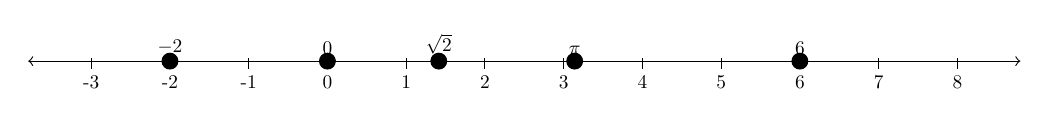
\begin{tikzpicture}[scale=1]
    \draw[<->] (-3.8,0) -- (8.8,0);
		\foreach \x in {-3,-2,-1,0,1,2,3,4,5,6,7,8} {\draw (\x,1pt) -- (\x,-3pt) node[anchor=north,scale=0.7] {\x};}
		\draw[fill=\blue]  (-2,0) circle (0.1); \node[above,scale=0.7] at (-2,0) {$-2$}; 
		\draw[fill=\blue]  (0,0) circle (0.1); \node[above,scale=0.7] at (0,0) {$0$}; 
		\draw[fill=\blue]  (1.414,0) circle (0.1); \node[above,scale=0.7] at (1.414,0) {$\sqrt{2}$}; 
		\draw[fill=\blue]  (3.14,0) circle (0.1); \node[above,scale=0.7] at (3.14,0) {$\pi$}; 
		\draw[fill=\blue]  (6,0) circle (0.1); \node[above,scale=0.7] at (6,0) {$6$}; 
    \end{tikzpicture}
\end{center}

Inequalities in real numbers translates to intervals along the real number line. For example:
\sitem{
\item The interval $-1 < x \leq 3$ translate too
\smallskip
\begin{center}
  \begin{tikzpicture}[scale=1]
    \draw[<->] (-3.8,0) -- (8.8,0);
		\foreach \x in {-3,-2,-1,0,1,2,3,4,5,6,7,8} {\node[dot=1,label=below:$\x$] at  (\x, 0) {}; }
		\draw[line width=0.8mm, \blue] (-1,0) -- (3,0); 
		\draw[fill=white]  (-1,0) circle (0.1); %\node[above] at (-3,0) {$-3$}; 
		\draw[fill=\blue]  (3,0) circle (0.1); %\node[above] at (2,0) {$2$}; 
    \end{tikzpicture}
 \end{center}

\item The interval $1\leq x < 6$ translates to
\smallskip
\begin{center}
  \begin{tikzpicture}[scale=1]
    \draw[<->] (-3.8,0) -- (8.8,0);
		\foreach \x in {-3,-2,-1,0,1,2,3,4,5,6,7,8} {\node[dot=1,label=below:$\x$] at  (\x, 0) {}; }
		\draw[line width=0.8mm,\blue] (1,0) -- (6,0); 
		\draw[fill=\blue]  (1,0) circle (0.1); %\node[above] at (2,0) {$2$}; 
		\draw[fill=white]  (6,0) circle (0.1); %\node[above] at (-3,0) {$-3$}; 
		\end{tikzpicture}
 \end{center}
}
\end{example}

We can extend this idea to complex numbers. Since two pieces of data is required to describe a complex number (a real part and an imaginary
part). We can use those two data as co-ordinates on the plane. The complex number $z = a+ib$ is represented by the point with co-ordinates $(a,b)$ in the plane. Complex numbers written in $z=a+ib$ is often called \emph{Cartesian form} for its connection with coordinates in the complex plane.

\begin{center}
\begin{tikzpicture}[scale=0.8]
	  \draw[<->] (-6.2,0) -- (6.2,0) ; \node[above] at (6.3,0) {$\RE{z}$};
    \draw[<->] (0,-4.2) -- (0,4.2) ; \node[right] at (0,4.3) {$\IM{z}$}; 
    	\foreach \x in {-6,-5,-4,-3,-2,-1,1,2,3,4,5,6}
     		\draw (\x,1pt) -- (\x,-3pt) node[anchor=north,scale=0.7] {\x};
    	\foreach \y in {-4,-3,-2,-1,1,2,3,4}
     		\draw (1pt,\y) -- (-3pt,\y) node[anchor=east,scale=0.7] {\y};
		\draw[fill=\blue]  (-5,3) circle (0.1) node[above] {$-5+3i$};
		\draw[fill=\blue]  (2,1) circle (0.1) node[above] {$2+i$};
		\draw[fill=\blue]  (-3,-3) circle (0.1) node[above] {$-3-3i$};
		\draw[fill=\blue]  (4,-2) circle (0.1) node[above] {$4-2i$};
\end{tikzpicture}
\end{center}

This is known as an \emph{Argand Diagram} or the \emph{complex plane}. The Argand diagram provides a simple visual way of representing many of the key properties of complex numbers.

\begin{example}
Let $z$ be a complex number. The Argand diagram of $\conj{z}$, the complex conjugate of $z$, is the point obtained by reflection in the real axis.
\begin{center}
\begin{tikzpicture}[scale=0.6]
	  \draw[<->] (-6.2,0) -- (6.2,0) ; \node[above,scale=0.7] at (6.3,0) {$\RE{z}$};
    \draw[<->] (0,-4.2) -- (0,4.2) ; \node[right,scale=0.7] at (0,4.3) {$\IM{z}$}; 
    	\foreach \x in {-6,-5,-4,-3,-2,-1,1,2,3,4,5,6}
     		\draw (\x,1pt) -- (\x,-3pt) node[anchor=north,scale=0.7] {\x};
    	\foreach \y in {-4,-3,-2,-1,1,2,3,4}
     		\draw (1pt,\y) -- (-3pt,\y) node[anchor=east,scale=0.7] {\y};
		\draw[fill=\blue]  (-5,3) circle (0.1) node[above] {$z$};
		\draw[fill=\blue]  (-5,-3) circle (0.1) node[above] {$\conj{z}$};
		\draw[fill=\blue]  (4,2) circle (0.1) node[above] {$\conj{w}$};
		\draw[fill=\blue]  (4,-2) circle (0.1) node[above] {$w$};
\end{tikzpicture}
\end{center}
\end{example}

\begin{exercise}{}
Plot all complex numbers of the form $z = a+3i$ for real numbers $a$
\end{exercise}
\begin{solution}

The imaginary part of $z$ is always 3 while the real part can vary. This leads to the following picture:

\begin{center}
\begin{tikzpicture}[scale=0.6]
	  \draw[<->] (-6.2,0) -- (6.2,0) ; \node[above,scale=0.7] at (6.3,0) {$\RE{z}$};
    \draw[<->] (0,-4.2) -- (0,4.2) ; \node[right,scale=0.7] at (0,4.3) {$\IM{z}$}; 
    	\foreach \x in {-6,-5,-4,-3,-2,-1,1,2,3,4,5,6}
     		\draw (\x,1pt) -- (\x,-3pt) node[anchor=north,scale=0.7] {\x};
    	\foreach \y in {-4,-3,-2,-1,1,2,4}
     		\draw (1pt,\y) -- (-3pt,\y) node[anchor=east,scale=0.7] {\y};
		\draw[<->, thick, \blue]  (-6,3) -- (6,3);
		\node[above,scale=0.7] at (4,3) {$z = a+3i$};
\end{tikzpicture}
\end{center}
\end{solution}

\begin{exercise}[label=ex:compcircle]{}
Plot all complex numbers $z = a+ib$ with the property that $a^2+b^2=9$.
\end{exercise}

\begin{solution}
Recall that $a^2+b^2=9$ is the equation of a circle with radius $3$. Thus a complex number $a+ib$ satisfies $a^2+b^2=9$ if it
lies on this circle.

\begin{center}
\begin{tikzpicture}[scale=0.6]
	  \draw[<->] (-6.2,0) -- (6.2,0) ; \node[above,scale=0.7] at (6.3,0) {$\RE{z}$};
    \draw[<->] (0,-4.2) -- (0,4.2) ; \node[right,scale=0.7] at (0,4.3) {$\IM{z}$}; 
    	\foreach \x in {-6,-5,-4,-3,-2,-1,1,2,3,4,5,6}
     		\draw (\x,1pt) -- (\x,-3pt) node[anchor=north,scale=0.7] {\x};
    	\foreach \y in {-4,-3,-2,-1,1,2,3,4}
     		\draw (1pt,\y) -- (-3pt,\y) node[anchor=east,scale=0.7] {\y};
		\draw[thick, \blue]  (0,0) circle (3);
		\node[scale=0.7] at (3,3) {$a^2+b^2=9$};
\end{tikzpicture}
\end{center}
Each point on the circle is a complex number satisfying the requirement.
\end{solution}

\begin{exercise}[label=ex:compcircle2]{}
Plot all complex numbers $z = a+ib$ with the property that 
$z \bar{z}=9$.
\end{exercise}

\begin{solution}
This is a retread of the previous question since $z \bar{z}= a^2+b^2=9$ is the equation of a circle with radius $3$. 

\begin{center}
\begin{tikzpicture}[scale=0.6]
	  \draw[<->] (-6.2,0) -- (6.2,0) ; \node[above,scale=0.7] at (6.3,0) {$\RE{z}$};
    \draw[<->] (0,-4.2) -- (0,4.2) ; \node[right,scale=0.7] at (0,4.3) {$\IM{z}$}; 
    	\foreach \x in {-6,-5,-4,-3,-2,-1,1,2,3,4,5,6}
     		\draw (\x,1pt) -- (\x,-3pt) node[anchor=north,scale=0.7] {\x};
    	\foreach \y in {-4,-3,-2,-1,1,2,3,4}
     		\draw (1pt,\y) -- (-3pt,\y) node[anchor=east,scale=0.7] {\y};
		\draw[thick, \blue]  (0,0) circle (3);
		\node[scale=0.7] at (3,3) {$a^2+b^2=9$};
\end{tikzpicture}
\end{center}

\end{solution}

%\tutorial{sec:compargand}

\secbreak \subsection{Polar Form}

Now that we have a visual representation of complex numbers, we can ask new questions about them. For example, what is the \emph{size} of a complex number. One way to define size is to take the distance between the number and the origin of the Argand diagram\footnote{This idea of using distance to origin as size is consistent with our knowledge \emph{vectors}}. 
\begin{center}
\begin{tikzpicture}[scale=0.6]
	  \draw[->] (-0.2,0) -- (6.2,0) ; \node[above,scale=0.7] at (6.3,0) {$\RE{z}$};
    \draw[->] (0,-0.2) -- (0,4.2) ; \node[right,scale=0.7] at (0,4.3) {$\IM{z}$}; 
		\draw[fill=\blue]  (5,3) circle (0.1) node[above] {$z=a+ib$};
		\draw[\blue,->] (0,0) -- node[above left] {$r$} ++ (5,3);
\end{tikzpicture}
\end{center}
Using Pythagoras' Theorem we get
\begin{align*}
r^2&=a^2+b^2 &r&=\sqrt{a^2+b^2}
\end{align*}

\begin{df}{Modulus}
The \emph{modulus} of the complex number $z =a+ib$ is denoted $\abs{z} = \abs{a+ib}$ and is defined by
\begin{align*}
\abs{z} &= \abs{a+ib} = \sqrt{a^2+b^2}
\end{align*}
\end{df}

\begin{exercise}{}
If $z=3-i$ calculate $\abs{z}$.
\end{exercise}
\begin{solution}
Since $z=a+ib$ with $a=3$ and $b=-1$, we have
\begin{align*}
\abs{z} &=\sqrt{3^2+(-1)^2} =\sqrt{10}
\end{align*}
\end{solution}


\begin{exercise}{}
Find the modulus of the following complex numbers
\senum{
\item $z = i$
\item $z = -9$,
\item $z = \abs{\frac{1}{\sqrt{2}}- \frac{1}{\sqrt{2}}i}$
}
\end{exercise}
\begin{solution}
Applying the theorem, we have
\senum{
\item $\abs{i}=\sqrt{0^2+1^2}=1$
\item $\abs{-9}=\sqrt{9^2+0^2}=9$
\item $\displaystyle \abs{\frac{1}{\sqrt{2}}- \frac{1}{\sqrt{2}}i}= \sqrt{\frac{1}{2}+\frac{1}{2}}=1.$
}
\end{solution}

\begin{exercise}{}
In the Argand diagram, draw the set of all complex numbers $z$ with modulus $\abs{z} = \sqrt{2}$.
\end{exercise}
\begin{solution}
A complex number $z = a+ib$ has modulus $\abs{z} = \sqrt{2}$ if $\sqrt{a^2+b^2}=\sqrt{2}$ or $a^2+b^2=2$ (See \autoref{ex:compcircle}).
\end{solution}

\begin{solution}
(Alternate) We know that the modulus of a complex number gives the distance to the origin. Thus we want all the points at distance $\sqrt2$ from the origin. This again leads to the circle of radius $\sqrt2$ (See \autoref{ex:compcircle}). 
\end{solution}

\begin{exercise}[label=ex:compareas]{}
Plot the set of complex numbers $z$ satisfying $1 < |z| \leq 2$ in the complex plane.
\end{exercise}
\begin{solution}
Since the modulus is the distance to the origin the set consists of all those complex numbers which are at a distance between $1$ and $2$ from the origin. This
gives the area shown below.

\begin{center}
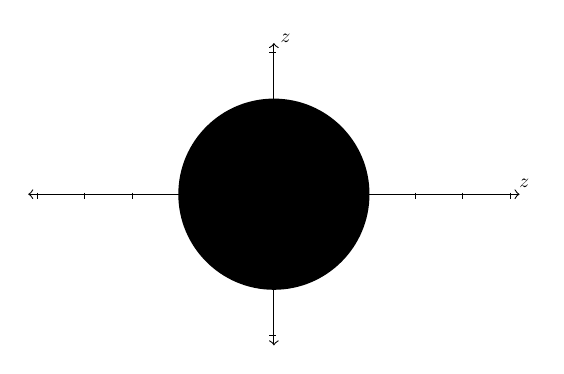
\begin{tikzpicture}[scale=0.6]
		\draw[fill=\gray, thick]  (0,0) circle (2);
		\draw[fill=\white, dashed, thick]  (0,0) circle (1);
	  \draw[<->] (-5.2,0) -- (5.2,0) ; \node[above,scale=0.7] at (5.3,0) {$\RE{z}$};
    \draw[<->] (0,-3.2) -- (0,3.2) ; \node[right,scale=0.7] at (0,3.3) {$\IM{z}$}; 
    	\foreach \x in {-5,-4,-3,-2,-1,1,2,3,4,5}
     		\draw (\x,1pt) -- (\x,-3pt);
    	\foreach \y in {-3,-2,-1,1,2,3}
     		\draw (1pt,\y) -- (-3pt,\y);
\end{tikzpicture}
\end{center}
\end{solution}
\caution Notice the difference between the inner and outer boundaries. A solid line indicates that the boundary is included and a dashed line indicates that the boundary is not included\footnote{This is analogous to using filled and hollowed circles to indicate endpoints of a real interval.}.

To uniquely define a complex number with the modulus, we would need another piece of information. This second piece of information is called the \emph{argument}.

\begin{df}[label=df:comparg]{(Principal) Argument}
Let $z$ be a complex number. The principal argument of $z$, denoted as $\Arg{z}$, is the angle $\theta$ in radians that $z$
makes with the positive real axis in a counter-clockwise direction, chosen so that $-\pi<\theta\leq\pi$.
\end{df}

A point $z$ in the Argand diagram determines an angle $\theta$ with the positive real axis.

\begin{center}
\begin{tikzpicture}[scale=0.8]
	  \draw[->] (-0.2,0) -- (6.2,0) ; \node[above,scale=0.7] at (6.3,0) {$\RE{z}$};
    \draw[->] (0,-0.2) -- (0,4.2) ; \node[right,scale=0.7] at (0,4.3) {$\IM{z}$}; 
		\draw[->] (0,0) -- (5,3);
		\draw[fill=\blue]  (5,3) circle (0.1) node[above] {$z$};
		\draw[\blue,->] (2,0) arc (0:31:2);
		\node[scale=0.7, \blue] at (2.2,0.5) {$\theta$};
\end{tikzpicture}
\end{center}

The choice of $\theta$ such that $-\pi<\theta\le\pi$ means:
\sitem{
\item $0 < \theta \leq \pi$ if $z$ is \emph{above} the real axis
\item $-\pi < \theta < 0$ if $z$ is \emph{below} the real axis
}

\begin{example}
The most straight forward method of determining the argument is to draw the diagram.

\begin{minipage}{0.5\textwidth}
\begin{center}
\begin{tikzpicture}[scale=0.4]
	  \draw[<->] (-6.2,0) -- (6.2,0) ; \node[above,scale=0.7] at (6.3,0) {$\RE{z}$};
    \draw[<->] (0,-4.2) -- (0,4.2) ; \node[right,scale=0.7] at (0,4.3) {$\IM{z}$}; 
		\draw[->,\blue] (0,0) -- (5,0);
		\draw[fill=\blue]  (5,0) circle (0.1) node[below] {$5$};
\end{tikzpicture}
\end{center}
\begin{center}
\begin{tikzpicture}[scale=0.4]
	  \draw[<->] (-6.2,0) -- (6.2,0) ; \node[above,scale=0.7] at (6.3,0) {$\RE{z}$};
    \draw[<->] (0,-4.2) -- (0,4.2) ; \node[right,scale=0.7] at (0,4.3) {$\IM{z}$}; 
		\draw[->,\blue] (0,0) -- (0,2);
		\draw[fill=\blue]  (0,2) circle (0.1) node[left] {$2i$};
		\draw[\blue,->] (1,0) arc (0:90:1);
\end{tikzpicture}
\end{center}

\end{minipage}%
\begin{minipage}{0.5\textwidth}
\begin{center}
\begin{tikzpicture}[scale=0.4]
	  \draw[<->] (-6.2,0) -- (6.2,0) ; \node[above,scale=0.7] at (6.3,0) {$\RE{z}$};
    \draw[<->] (0,-4.2) -- (0,4.2) ; \node[right,scale=0.7] at (0,4.3) {$\IM{z}$}; 
		\draw[->,\blue] (0,0) -- (-3,0);
		\draw[fill=\blue]  (-3,0) circle (0.1) node[below] {$3$};
		\draw[\blue,->] (1,0) arc (0:180:1);
\end{tikzpicture}
\end{center}
\begin{center}
\begin{tikzpicture}[scale=0.4]
	  \draw[<->] (-6.2,0) -- (6.2,0) ; \node[above,scale=0.7] at (6.3,0) {$\RE{z}$};
    \draw[<->] (0,-4.2) -- (0,4.2) ; \node[right,scale=0.7] at (0,4.3) {$\IM{z}$}; 
		\draw[->,\blue] (0,0) -- (0,-4);
		\draw[fill=\blue]  (0,-4) circle (0.1) node[left ] {$-4i$};
		\draw[\blue,->] (1,0) arc (0:-90:1);
\end{tikzpicture}
\end{center}
\end{minipage}

Based on the diagrams, we have:
\begin{align*}
\Arg{5}&=0 & \Arg{-3}&=\pi\\
\Arg{2i}&=\frac{\pi}{2} & \Arg{-4i}&=-\frac{\pi}{2}
\end{align*}

A similar approach would show that
\begin{align*}
\Arg{1+i} &=\frac{\pi}{4}&
\Arg{-1+i}&=\frac{3\pi}{4}\\
\Arg{1-i} &=-\frac{\pi}{4}&
\Arg{-1-i}&=-\frac{3\pi}{4}
\end{align*}
\end{example}



\begin{example}
We can use our knowledge of coordinate axes to determine:
\begin{align*}
\Arg{1} &=0&
\Arg{i}&=\frac{\pi}{2}\\
\Arg{-1} &=\pi&
\Arg{-i}&=-\frac{\pi}{2}
\end{align*}
Further, we can use the special triangles to get
\begin{align*}
\Arg{\sqrt{3}+i} &=\frac{\pi}{6}&
\Arg{1+i\sqrt{3}} &=\frac{\pi}{3}
\end{align*}
\end{example}

These are all cases we can obtain the angles by drawing and using our experience with simple triangles. We can extend this and develop a more systematic method to use for more general complex numbers

\begin{example}
Suppose $z=a+ib$ is a complex number which determines an angle $\theta$ with the real axis. 

\begin{center}
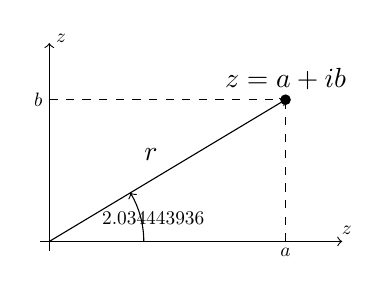
\begin{tikzpicture}[scale=0.6]
	  \draw[->] (-0.2,0) -- (6.2,0) ; \node[above,scale=0.7] at (6.3,0) {$\RE{z}$};
    \draw[->] (0,-0.2) -- (0,4.2) ; \node[right,scale=0.7] at (0,4.3) {$\IM{z}$}; 
		\draw[\blue,->] (0,0) -- node[above left] {$r$} ++ (5,3);
		\draw[dashed] (5,0) -- (5,3);
		\draw[dashed] (0,3) -- (5,3);
		\node[left,scale=0.7] at (0,3) {$b$}; 
		\node[below,scale=0.7] at (5,0) {$a$}; 
		\draw[fill=\blue]  (5,3) circle (0.1) node[above] {$z=a+ib$};
		\draw[\blue,->] (2,0) arc (0:31:2);
		\node[scale=0.7, \blue] at (2.2,0.5) {$\theta$};
\end{tikzpicture}
\end{center}


We can use our knowledge of trigonometry to get that
\begin{equation*}
\tan(\theta) = \frac{b}{a}
\end{equation*}
In order words, we can determine the argument $\theta$ from the Cartesian form. 
\end{example}

\caution In the case where $a=0$, we are on the imaginary axis and can resolve the angle using more simple methods.

\begin{exercise}{}
Find $\Arg{1+2i}$.
\end{exercise}

\begin{solution}
We start by plotting a diagram 

\begin{center}
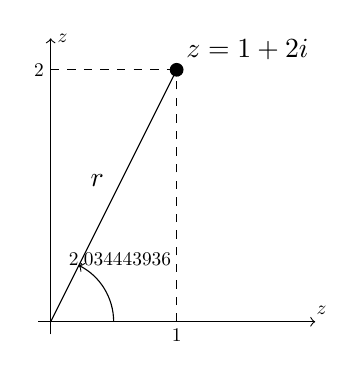
\begin{tikzpicture}[scale=0.8]
	  \draw[->] (-0.2,0) -- (4.2,0) ; \node[above,scale=0.7] at (4.3,0) {$\RE{z}$};
    \draw[->] (0,-0.2) -- (0,4.5) ; \node[right,scale=0.7] at (0,4.5) {$\IM{z}$}; 
		\draw[\blue,->] (0,0) -- node[above left] {$r$} ++ (2,4);
		\draw[dashed] (2,0) -- (2,4);
		\draw[dashed] (0,4) -- (2,4);
		\node[left,scale=0.7] at (0,4) {$2$}; 
		\node[below,scale=0.7] at (2,0) {$1$}; 
		\draw[fill=\blue]  (2,4) circle (0.1) node[above right] {$z=1+2i$};
		\draw[\blue,->] (1,0) arc (0:63.5:1);
		\node[scale=0.7, \blue] at (1.1,1) {$\theta$};
\end{tikzpicture}
\end{center}

Using the above formula we know that $\tan(\theta)=\frac{2}{1} = 2$. Using a calculator we get 
\begin{equation*}
\theta =\arctan(2) = 1.107
\end{equation*}
to 3 decimal places (in radians!).

\end{solution}
\caution Even though we have $\tan(\theta) = \frac{b}{a}$, we have cases where $\theta \neq \arctan\left(\frac{b}{a}\right)$.


\begin{example}
Suppose we want to find $\Arg{-1-2i}$ using the same method. We will that $\frac{b}{a}  = \frac{-2}{-1} =2$, which will give $\theta =\arctan(2) = 1.107$. However this is clearly not correct based on our previous exercise. That is $w=-1-2i$ and $z=1+2i$ are not in the same direction.

\end{example}

The reason for this is because the inverse tangent function produces values $-\frac{\pi}{2} < \theta < \frac{\pi}{2}$. In other words, the it assumes $a >0$. If we want to obtain the argument for the complex number in the exact opposite direction, we have to account for it by adding or subtracting $\pi$

\begin{example}
Consider the numbers $z = 1+i$ and $w = -1-i$. We know $\Arg{z} = \frac{\pi}{4}$ and $\Arg{w} = -\frac{3\pi}{4}$  and $\tan\left(\frac{\pi}{4}\right) = \tan\left(\frac{-3\pi}{4}\right)=1$. If we plot a diagram, we see why this is the case and how we can resolve it.

\begin{center}
\begin{tikzpicture}[scale=0.8]
	  \draw[->] (-4.2,0) -- (4.2,0) ; \node[above,scale=0.7] at (4.3,0) {$\RE{z}$};
    \draw[->] (0,-3.2) -- (0,3.5) ; \node[right,scale=0.7] at (0,3.5) {$\IM{z}$}; 
		\draw[\blue,->] (0,0) -- (2,2);
		\draw[\red ,->] (0,0) -- (-2,-2);
		\draw[\blue,->] (1,0) arc (0:45:1);
		\draw[\red ,->] (1,0) arc (0:-135:1);
		\draw[->] (0.5,0) arc (0:-135:0.5);
		\draw[->] (0.5,0) arc (0:45:0.5);
		\draw[fill=\blue]  (2,2) circle (0.1) node[above right] {$z$};
		\draw[fill=\red ]  (-2,-2) circle (0.1) node[below left] {$w$};
		\node[scale=0.7] at (0.5,-0.5) {$\pi$};
		\node[scale=0.7, \blue] at (1.1,0.5) {$\frac{\pi}{4}$};
		\node[scale=0.7, \red] at (-0.6,-1.3) {$\frac{-3\pi}{4}$};
\end{tikzpicture}
\end{center}

Be sure to have your calculator set to \textbf{radians} mode 
\end{example}

\begin{thm}[title= Summary \thethm\;]{}
To find $\theta =\Arg{a+ib}$, 
\begin{enumerate}
\item Draw a picture showing the angle. Stop if the angle is from a special triangle or on the axes.
\item Determine which {\it quadrant} the point is in and use the following:
\end{enumerate}
\begin{center}
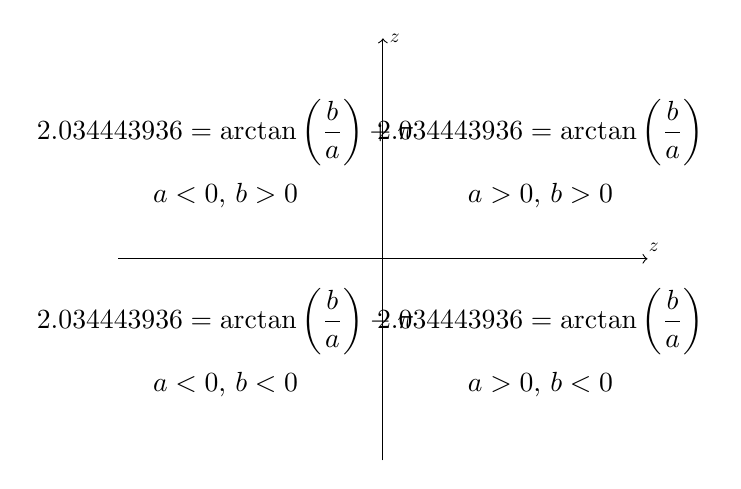
\begin{tikzpicture}[scale=0.8]
	  \draw[->] (-4.2,0) -- (4.2,0) ; \node[above,scale=0.7] at (4.3,0) {$\RE{z}$};
    \draw[->] (0,-3.2) -- (0,3.5) ; \node[right,scale=0.7] at (0,3.5) {$\IM{z}$}; 
		\node[scale=1] at (-2.5,2.0) {$\displaystyle \theta =\arctan\left(\frac{b}{a}\right)+\pi$};
		\node[scale=1] at (-2.5,1.0) {$a<0$, $b>0$};
		\node[scale=1] at (2.5,2.0) {$\displaystyle \theta =\arctan\left(\frac{b}{a}\right)$};
		\node[scale=1] at (2.5,1.0) {$a>0$, $b>0$};
		\node[scale=1] at (-2.5,-1.0) {$\displaystyle \theta =\arctan\left(\frac{b}{a}\right)-\pi$};
		\node[scale=1] at (-2.5,-2.0) {$a<0$, $b<0$};
		\node[scale=1] at (2.5,-1.0) {$\displaystyle \theta =\arctan\left(\frac{b}{a}\right)$};
		\node[scale=1] at (2.5,-2.0) {$a>0$, $b<0$};
\end{tikzpicture}
\end{center}

The four {\it quadrants} of the complex plane are usually numbered anti-clockwise.

% Four quadrants in the complex plane (Argand diagram), labelled I–IV.
% Style: clean axes with arrows, light quadrant shading, roman numerals.
\begin{center}
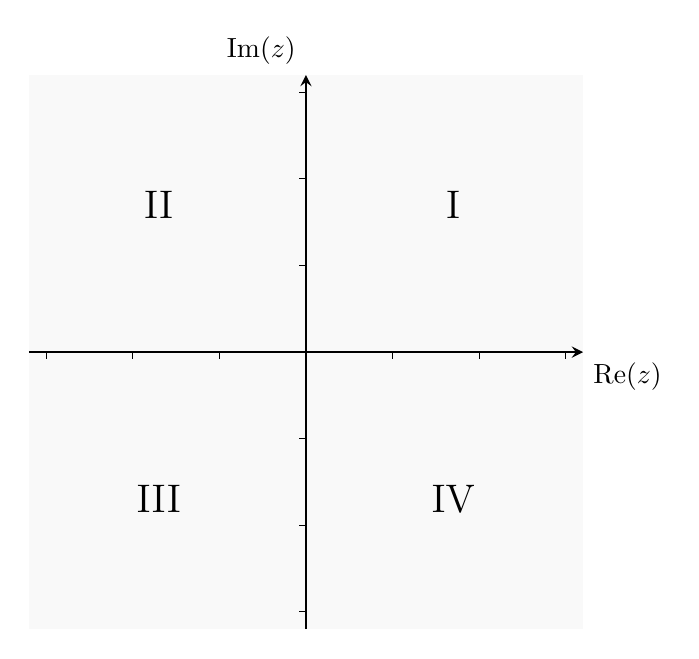
\begin{tikzpicture}[scale=1.1,>=stealth]
  % Axes limits
  \def\xmax{3.2}
  \def\ymax{3.2}

  % Light quadrant shading (optional; comment out if you prefer white)
  \fill[gray!05] (0,0) rectangle (\xmax,\ymax);      % QI
  \fill[gray!05] (-\xmax,0) rectangle (0,\ymax);     % QII
  \fill[gray!05] (-\xmax,-\ymax) rectangle (0,0);    % QIII
  \fill[gray!05] (0,-\ymax) rectangle (\xmax,0);     % QIV

  % Axes
  \draw[->,thick] (-\xmax,0) -- (\xmax,0) node[below right] {Re$(z)$};
  \draw[->,thick] (0,-\ymax) -- (0,\ymax) node[above left] {Im$(z)$};

  % Tick marks (minimal)
  \foreach \t in {-3,-2,-1,1,2,3}{
    \draw (\t,0) -- (\t,-0.08);
    \draw (0,\t) -- (-0.08,\t);
  }

  % Quadrant labels (roman numerals)
  \node at ( 1.7, 1.7) {\Large I};
  \node at (-1.7, 1.7) {\Large II};
  \node at (-1.7,-1.7) {\Large III};
  \node at ( 1.7,-1.7) {\Large IV};

  % Dashed lines for the axes (optional; uncomment if your notes use them)
  % \draw[dashed,gray] (-\xmax,0) -- (\xmax,0);
  % \draw[dashed,gray] (0,-\ymax) -- (0,\ymax);
\end{tikzpicture}
\end{center}




\end{thm}

\newpage
\begin{exercise}[label=ex:comparg]{}
Find $\Arg{-1+2i}$. 
\end{exercise}
\begin{solution}
Starting with the picture:

%\insf{another damned picture} - Kept original comment. -Tom
\begin{center}
\begin{tikzpicture}[scale=0.8]
	  \draw[->] (-2.2,0) -- (2.2,0) ; \node[above,scale=0.7] at (2.3,0) {$\RE{z}$};
    \draw[->] (0,-0.2) -- (0,3.5) ; \node[right,scale=0.7] at (0,3.5) {$\IM{z}$}; 
		\draw[\blue,->] (0,0) -- node[below left] {$r$} ++ (-1,2);
		\draw[fill=\blue]  (-1,2) circle (0.1) node[above left] {$z=-1+2i$};
		\draw[\blue,->] (0.5,0) arc (0:116.5:0.5);
		\node[scale=0.7, \blue] at (0.5,0.5) {$\theta$};
\end{tikzpicture}
\end{center}
We see that $0<\Arg{-1+2i} <\pi$. Using the above formula we know that $\tan(\theta)=\frac{2}{-1}=-2$. Using a calculator we get
\begin{equation*}
\arctan(-2)=-1.107
\end{equation*}
to 3 decimal places. Since this is not in the correct range for $\theta$. Adding $\pi$ gives
\begin{equation*}
\theta = -1.107+\pi = 2.034
\end{equation*}

\end{solution}



\begin{exercise}{}
Find $\Arg{3-4i}$.
\end{exercise}
\begin{solution}
We see that $-\frac{\pi}{2}<\Arg{3-4i}<0$, so the inverse tangent value should give us the right argument. This gives:
\begin{equation*}
\Arg{3-4i}=\arctan\left(\frac{-4}{3}\right)= -0.927.
\end{equation*}
\end{solution}

Now that we have we can determine the modulus and argument of a complex number, we can try to reverse the process.

\begin{df}{Polar form}
Let $z$ be a complex number with modulus $r$ and principal argument $\theta$. The polar form of $z$ is given by
\begin{align*}
z &= r\cos(\theta) + i r\sin(\theta)\\
&= r\left(\cos(\theta) + i\sin(\theta)\right)
\end{align*}
\end{df}

We can verify this by looking at the picture and applying a bit of trigonometry.
\begin{center}
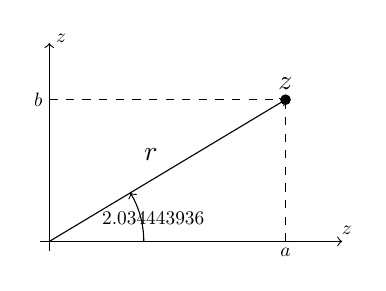
\begin{tikzpicture}[scale=0.6]
	  \draw[->] (-0.2,0) -- (6.2,0) ; \node[above,scale=0.7] at (6.3,0) {$\RE{z}$};
    \draw[->] (0,-0.2) -- (0,4.2) ; \node[right,scale=0.7] at (0,4.3) {$\IM{z}$}; 
		\draw[\blue,->] (0,0) -- node[above left] {$r$} ++ (5,3);
		\draw[dashed] (5,0) -- (5,3);
		\draw[dashed] (0,3) -- (5,3);
		\node[left,scale=0.7] at (0,3) {$b$}; 
		\node[below,scale=0.7] at (5,0) {$a$}; 
		\draw[fill=\blue]  (5,3) circle (0.1) node[above] {$z$};
		\draw[\blue,->] (2,0) arc (0:31:2);
		\node[scale=0.7, \blue] at (2.2,0.5) {$\theta$};
\end{tikzpicture}
\end{center}

From the picture, we see that the base $a = r\cos(\theta)$ and height $b = r\sin(\theta)$. Hence, we have
\begin{equation*}
z =r\cos(\theta)+i r\sin(\theta)
\end{equation*}

\begin{exercise}{}
Suppose $\abs{z}=2$ and $\Arg{z}=\frac{\pi}{3}$. Write $z$ in polar form.
\end{exercise}
\begin{solution}
Set $r=\abs{z}=2$ and $\theta=\Arg{z}=\frac{\pi}{3}$. Then
\begin{align*}
z&= r\left(\cos(\theta)+i\sin(\theta)\right)\\
 &= 2\left(\cos\left(\frac{\pi}{3}\right)+i\sin\left(\frac{\pi}{3}\right)\right)
\end{align*}
\end{solution}
If we wished to convert it to Cartesian form, we can further simplify
\begin{align*}
z&= 2\left(\cos\left(\frac{\pi}{3}\right)+i\sin\left(\frac{\pi}{3}\right)\right)\\
 &= 2\left(\frac{1}{2}+i\frac{\sqrt{3}}{2}\right)\\
 &= 1+i\sqrt{3}
\end{align*}

In general, if we want to write a complex number in polar form, we:
\begin{enumerate}
\item Compute the modulus, $r=\abs{z}$.
\item Computer the principal argument, $\theta=\Arg{z}$.
\item Write $z$ as
\begin{equation*}
z= r\left(\cos(\theta)+i\sin(\theta)\right)\\
\end{equation*}
\end{enumerate}

We will see in the next subsection that we can also write this as $z = r\, e^{i\theta}$.

\begin{exercise}[label=ex:1ipolar]{}
Write $z= 1+i$ in polar form.
\end{exercise}
\begin{solution}
First we calculate the modulus and principal argument.
\sitem{
\item Modulus: $\abs{z}=\sqrt{1^2+1^2}=\sqrt{2}$.
\item Principal Argument: $\Arg{z}=\arctan\left(\frac{1}{1}\right) = \frac{\pi}{4}$. Since $z$ is in the first quadrant, the argument does not need altering. 
}
Thus the polar form of $z= 1+i$ is
\begin{equation*}
z = \sqrt{2} \left(\cos\left(\frac{\pi}{4}\right)+i\sin\left(\frac{\pi}{4}\right)\right)
\end{equation*}
\end{solution}

\begin{exercise}{}
Write $z=-1+2i$ in polar form.
\end{exercise}
\begin{solution}
First we calculate the modulus and principal argument.
\sitem{
\item Modulus: $\abs{z}=\sqrt{(-1)^2+2^2}=\sqrt{5}$.
\item Principal Argument: $\Arg{z}=\arctan\left(\frac{2}{-1}\right) = -1.107$. Since $z$ is in the upper-left quadrant, we need to alter the argument (see \autoref{ex:comparg}) to get $\Arg{z} = 2.034$
}
Thus the polar form of $z= -1+2i$ is
\begin{equation*}
z = \sqrt{5} \left(\cos\left(2.034\right)+i\sin\left(2.034\right)\right)
\end{equation*}
\end{solution}

%\tutorial{sec:comppolar}

\secbreak \subsection{Exponential Form} 

The introduction of complex numbers connects two key areas of mathematics: Trigonometry and the exponential. It is possible to write a Maclaurin series for the exponential
\begin{equation*}
e^x = 1+x+\frac{x^2}{2!}+\frac{x^3}{3!} + \cdots = \sum_{n=0}^{\infty} \frac{x^n}{n!}
\end{equation*}

As it turns out, the exponential can be extended to complex numbers in the analogous way.

\begin{df}{Complex exponential}
For a complex number $z$, the complex exponential is defined to be:
\begin{equation*}
e^z = 1+z+\frac{z^2}{2!}+\frac{z^3}{3!} + \cdots = \sum_{n=0}^{\infty} \frac{z^n}{n!}
\end{equation*}
\end{df}

It is not at all obvious, but it is a fact that the infinite summation results in something finite for all complex $z$ so long as $|z|<\infty$.

If we consider the complex number $z=i\theta$ for an angle $\theta$, we get:
\begin{align*}
e^{i\theta} &= 1+\left(i\theta\right)+\frac{\left(i\theta\right)^2}{2!}+\frac{\left(i\theta\right)^3}{3!} + \cdots = \sum_{n=0}^{\infty} \frac{\left(i\theta\right)^n}{n!}
\end{align*}
By resolving the powers of $i$, we get
\begin{align*}
e^{i\theta} &= 1+\left(i\theta\right)+\frac{\left(i\theta\right)^2}{2!}+\frac{\left(i\theta\right)^3}{3!} + \frac{\left(i\theta\right)^4}{4!} + \frac{\left(i\theta\right)^5}{5!} + \cdots \\
&= 1+i\theta - \frac{\theta^2}{2!} -\frac{i\theta^3}{3!} + \frac{\theta^4}{4!} + \frac{i\theta^5}{5!} + \cdots\\
&= \left(1- \frac{\theta^2}{2!} + \frac{\theta^4}{4!} + \cdots \right) + i \left(\theta - \frac{\theta^3}{3!} + \frac{\theta^5}{5!} + \cdots\right)
\end{align*}
Recalling the Maclaurin series for $\sin(x)$ and $\cos(x)$ , we see that the two summations give:
\begin{align*}
e^{i\theta} &= \cos(\theta) + i \sin(\theta)
\end{align*}

This gives a fundamental result in complex numbers

\begin{thm}{Euler's Formula}
For any angle $\theta$, we have 
\begin{equation*}
e^{i\theta} = \cos(\theta) + i \sin(\theta)
\end{equation*}
\end{thm}

In particular, if $\theta =\pi$, we have the famous equation\footnote{This remarkable formula was obtained by Leonhard Euler in around 1768. The special case (one of the Top 10 equations ever!) links 5 fundamentally important numbers: $1$,$0$, $e$, $\pi$ and $i$ that have their origin in different branches of mathematics.}
\begin{equation*}
e^{i\pi} +1 = 0
\end{equation*}

\begin{example}
With Euler's formula, we have
\begin{align*}
e^{i1} &= \cos(1)+i\sin(1).\\
e^{i\frac{\pi}{2}} &= \cos\left(\frac{\pi}{2}\right)+i\sin\left(\frac{\pi}{2}\right) = 0 + 1i = i.
\end{align*}
\end{example}

Using Euler's formula we can get a new and very useful representation for complex numbers in polar form.

\begin{df}{Exponential form}
The exponential form of the complex number $z$ with modulus $r$ and argument $\theta$ is written as
\begin{equation*}
z = re^{i\theta}
\end{equation*}
\end{df}

We derive this form by applying Euler's Formula to the polar form
\begin{equation*}
z= r\left(\cos(\theta)+i\sin(\theta)\right) = re^{i\theta}
\end{equation*}

To write a complex number $z$ in exponential form:
\begin{enumerate}
\item Calculate the modulus $r = \abs{z}$,
\item Calculate the principle argument $\theta = \Arg{z}$,
\item Write $z=re^{i\theta}$.
\end{enumerate}


\begin{exercise}{}
Write $z = 1+i$ in exponential form.
\end{exercise}
\begin{solution}
Building on \autoref{ex:1ipolar}, we know $\abs{z}= \sqrt{2}$ and $\Arg{z}=\frac{\pi}{4}$.
Hence, the exponential form is
\begin{equation*}
z = 1+i= \sqrt2 e^{i\frac{\pi}{4}}.
\end{equation*}
\end{solution}

\begin{exercise}{}
\question Write $-i$ and $-1$ in exponential form.
\end{exercise}

Now that we have shown how to convert a complex number from Cartesian form $a+ib$ to exponential form $r e^{i\theta}$, we can go in the reverse direction.

\begin{exercise}{}
Write the complex number $z=2e^{i\frac{\pi}{4}}$ in Cartesian form $a+ib$.
\end{exercise}

\begin{solution}
Using Euler's formula, we have
\begin{align*}
z &= 2e^{i\frac{\pi}{4}}\\
&=2\left(\cos\left(\frac{\pi}{4}\right)+i\sin\left(\frac{\pi}{4}\right)\right) \\
&=2\left(\frac{1}{\sqrt{2}}+i\frac{1}{\sqrt{2}}\right)\\
&=\sqrt{2}+i \sqrt{2}
\end{align*}
\end{solution}

\begin{exercise}{}
Let $z=5+4i$. Write $e^z$ in the form $a+ib$.
\end{exercise}

\begin{solution}
We have (to 2 decimal point)
\begin{align*}
e^{5+4i} &= e^5e^{4i}\\
&= e^5\left(\cos(4)+i\sin(4)\right)\\
&=e^5\cos(4)+ie^5\sin(4)\\
&\approx -97.01-112.32i
\end{align*}
\end{solution}

Recall that multiplication and division of complex numbers can be quite an involved process (See \autoref{ex:compdiv}). However, we can utilise properties of the exponential function (and hence the exponential form) help simplify this process.

Let $z$ and $w$ be complex numbers. Then we have:
\begin{align*}
e^z\cdot e^w&=e^{z+w}  & \frac{e^z}{e^w} &=e^{z-w}  
\end{align*}

We can express this as:

\begin{thm}[label=thm:compmult]{Multiplication and division in exponential form}
Let $z = re^{i\theta}$ and $w = se^{i\phi}$ be complex numbers in exponential form
\begin{align*}
z\cdot w &= (r\cdot s) e^{i(\theta+\phi)} & \frac{z}{w} &= \frac{r}{s} e^{i(\theta-\phi)}.
\end{align*}
Converting the right-hand side to \emph{polar form} gives:
\begin{align*}
z\cdot w &= (r\cdot s) \left(\cos(\theta+\phi) + i \sin(\theta+\phi)\right) \\
\frac{z}{w} &= \frac{r}{s} \left(\cos(\theta-\phi) + i \sin(\theta-\phi)\right).
\end{align*}
\end{thm}

\begin{exercise}{}
Let $z=2e^{\frac{i \pi}{4}}$, and $w=e^{-\frac{i \pi}{4}}$. Find $z\cdot w$ and $\frac{z}{w}$.
\end{exercise}
\begin{solution}
Reading off the complex numbers, we get $r=2, s=1, \theta=\frac{\pi}{4}, \phi=-\frac{\pi}{4}$. So we get:
\begin{align*}
z\cdot w &= (2\cdot 1) \left[\cos\left(\frac{\pi}{4}+\left(-\frac{\pi}{4}\right)\right) + i \sin\left(\frac{\pi}{4}+\left(-\frac{\pi}{4}\right)\right)\right]\\
&=2\left[\cos(0)+i \sin(0)\right]=2\\
\frac{z}{w} &= \frac{2}{1} \left[\cos\left(\frac{\pi}{4}-\left(-\frac{\pi}{4}\right)\right) + i \sin\left(\frac{\pi}{4}-\left(-\frac{\pi}{4}\right)\right)\right]\\
&= \frac{2}{1} \left[\cos(\pi/2) + i \sin(\pi/2)\right] = 2i.
\end{align*}
\end{solution}

Complex exponentials are extremely useful when dealing with multiplication and division\footnote{but not so effective when dealing with addition and subtraction.}. However, its usefulness extends beyond simple arithmetic. For the rest of this section, we will take a (very brief) look into areas where complex exponentials might be useful.

\subsubsection*{Complex exponentials and trigonometric functions}

Euler's formula gives us an alternative way to write the sine and cosine functions which is used very widely in science and engineering. In particular, we have
\begin{align*}
e^{i\theta} + e^{-i\theta}  &= \left(\cos(\theta) + i \sin(\theta)\right) + \left(\cos(\theta) - i \sin(\theta)\right) = 2 \cos(\theta)\\
e^{i\theta} - e^{-i\theta}  &= \cos(\theta) + i \sin(\theta) - \left(\cos(\theta) - i \sin(\theta)\right) = 2 i \sin(\theta)
\end{align*}

We can rearrange to get the following:
\begin{thm}{Trigonometric functions in exponential forms}
We can express the trigonometric functions:
\begin{align*}
\cos(\theta) &= \frac{1}{2}\left(e^{i\theta} + e^{-i\theta}\right),\\
\sin(\theta) &= \frac{1}{2i}\left(e^{i\theta} - e^{-i\theta}\right).
\end{align*}
\end{thm}

Notice that these relations are very similar to the ones for the hyperbolic trigonometric functions (cosh and sinh). The introduction of complex numbers illustrates why they share so many similar identities.

\begin{exercise}{}
\question Use complex exponentials to show that $2\sin(\theta)\cos(\theta)=\sin(2\theta)$.
\end{exercise}

\subsubsection*{Calculus with complex exponentials}

The complex exponential is also commonly involved in the solution of differential equations, particularly in cases where solutions oscillate (like in AC electronics, quantum mechanics, etc.). It satisfies the same rules of differentiation and integration as any other exponential function\footnote{In essence, we can treat the complex number $i$ like a constant.}.

\begin{example}
For derivatives involving $i$, we have
\begin{align*}
\frac{d}{dx} e^{i \omega x} &= i \omega e^{i \omega x} \\
\frac{d^2}{dx^2} e^{i \omega x} &= (i \omega)^2 e^{i \omega x} = -\omega^2 e^{i \omega x}
\end{align*}
Integration works in a similar way
\begin{align*}
\int e^{i \omega x} dx &= \frac{e^{i \omega x}}{i\omega} + C
\end{align*}
\end{example}

\begin{exercise}{}
\question Verify that $y(t) = C e^{-i4t}$ is a solution of $y'' = -16 y$.
\end{exercise}

\subsubsection*{Logarithms of complex numbers}

Now that we have seen the exponential in complex numbers, it is natural to question how logarithm behave in complex numbers? The short answer is that logarithms are very complicated beasts, with properties far beyond this introductory course. \caution Use with caution! 

Suppose we ``naively'' apply logarithms on complex numbers using the rules of real numbers, we have the following.

\begin{example}
Let $z = r e^{i\theta}$ be a complex number in exponential form. We can apply the logarithm as
\begin{align*}
\Log(z) &= \Log\left(r e^{i\theta}\right)\\
&= \Log\left(r\right) + \Log\left(e^{i\theta}\right)\\
&= \Log\left(r\right) + i\theta\\
&= \Log\abs{z} + i\Arg{z}
\end{align*}
\end{example}

\begin{exercise}{}
Let $z = 42 e^{i\frac{\pi}{7}}$. Find $\Log(z)$.
\end{exercise}
\begin{solution}
Since $|z| = 42$ and $\Arg{z} = \frac{\pi}{7}$, we have $\Log(z) = \Log(42) + i\frac{\pi}{7}$.
\end{solution}

\caution Whilst this approach is not wrong, it also does not capture the entire picture\footnote{Recall from \autoref{df:comparg} that we have $-\pi < \Arg{z} \leq \pi$. However, this is a choice we made and there are other (non-principal) arguments we can take to be the angle of a complex number. For example, we could have chosen $0 < \Arg{z} \leq 2\pi$, which would affect the resulting logarithm.}.

%\tutorial{sec:compexponential}

\secbreak \subsection{De Moivre's Theorem}

Through repeated application of \autoref{thm:compmult}, we can extend exponential multiplication to powers of exponentials. We start with
\begin{equation*}
e^{i\theta} \cdot e^{i\theta} = e^{i (\theta+\theta)} = e^{i 2\theta}
\end{equation*}
which can be extended to any integer $n$ giving
\begin{equation*}
\left(e^{i\theta}\right)^n = e^{i n\theta}
\end{equation*}

If we convert both sides of the above equation into polar form, we obtain a very important result.

\begin{thm}{De Moivre's Theorem}
Let $n$ be an integer. For an angle $\theta$, we have
\begin{equation*}
\left(\cos(\theta)+i\sin(\theta)\right)^n = \cos(n\theta) +i\sin(n\theta).
\end{equation*}
For a complex number $z = r e^{i\theta}$ in exponential form, the following are equivalent
\begin{align*}
z^n &=  r^n e^{i n\theta} = r^n \left(\cos(n\theta) + i \sin(n\theta)\right)\\
&=  r^n \left(e^{i\theta}\right)^n = r^n \left(\cos(\theta)+i\sin(\theta)\right)^n
\end{align*}
\end{thm}

De Moivre's Theorem is particularly useful when dealing with powers of complex numbers. 

\begin{exercise}{}
Let $z=(1+i)$ and compute $z^8$
\end{exercise}

\begin{solution}
We first write $z$ in expontial form as
\begin{equation*}
z = 1+i=\sqrt{2} \left(\cos\left(\frac{\pi}{4}\right)+i\sin\left(\frac{\pi}{4}\right)\right) = \sqrt{2}e^{i\frac{\pi}{4}}
\end{equation*}
This gives
\begin{align*}
z^8 &= (1+i)^8\\
& = \left(\sqrt{2}e^{i\frac{\pi}{4}}\right)^8\\
& = \sqrt{2}^8 e^{i\frac{8\pi}{4}}\\
&= 16 e^{i2\pi}=16
\end{align*}
\end{solution}

We can reach the same solution by multiplying 8 times. But this would be rather tedious and not recommended.

\begin{exercise}{}
Compute $(-1+2i)^{10}$
\end{exercise}
\begin{solution}
Putting $z= (-1+2i)$ in exponential form, we find
\begin{equation*}
z= (-1+2i)=\sqrt{5}\big(\cos(2.034)+i \sin(2.034)\big) = \sqrt{5}e^{2.034i}
\end{equation*}
Thus we have
\begin{equation*}
z^{10} = (-1+2i)^{10} = \left(\sqrt{5}e^{2.034i}\right)^{10} = 3125 e^{20.34i} = 250.8+ 3115i
\end{equation*}
\end{solution}

De Moivre's theorem is also useful for computing roots of complex numbers.

\begin{thm}[label=thm:comproot]{Roots of complex numbers}
Let $z = r\, e^{i\theta}$ be a complex number in exponential form and $n$ be a positive integer. There are precisely $n$ different $n$-th roots of $z$ and they are given by
\begin{align*}
        z^{\frac{1}{n}} &= r^{\frac{1}{n}} e^{i \frac{\theta + 2\pi k}{n}}  &\text{for\;} k=0,1,\ldots,n-1
\end{align*}
where $r^{\frac{1}{n}}$ is the positive $n$-th root of $r$.
\end{thm}

\begin{example}
For \emph{square roots} of $z = re^{i\theta}$ we have $n=2$. So the \emph{two roots} $w_1, w_2$ are given by
\begin{align*}
w_1 &= \sqrt{r} e^{i\frac{\theta + 2\pi 0}{2}} = \sqrt{r} e^{i\frac{\theta}{2}}\\
w_2 &= \sqrt{r} e^{i\frac{\theta + 2\pi 1}{2}} = \sqrt{r} e^{i\frac{\theta + 2\pi}{2}}
\end{align*}
and $\sqrt{r}$ is the positive square root of $r$.

For \emph{cube roots} of $z = re^{i\theta}$ we have $n=3$. So the \emph{three roots} $w_1, w_2, w_3$ are given by
\begin{align*}
w_1 &= \sqrt[3]{r} e^{i\frac{\theta + 2\pi 0}{3}} = \sqrt[3]{r} e^{i\frac{\theta}{3}}\\
w_2 &= \sqrt[3]{r} e^{i\frac{\theta + 2\pi 1}{3}} = \sqrt[3]{r} e^{i\frac{\theta + 2\pi}{3}}
w_3 &= \sqrt[3]{r} e^{i\frac{\theta + 2\pi 2}{3}} = \sqrt[3]{r} e^{i\frac{\theta + 4\pi}{3}}
\end{align*}
and $\sqrt[3]{r}$ is the positive cubed root of $r$.
\end{example}


\begin{exercise}{}
Let $z = 9e^{i\frac{\pi}{3}}$. Find the two values of $\sqrt{z}$ and verify your answer.
\end{exercise}
\begin{solution}
Apply \autoref{thm:comproot} with $r=9$, $\theta = \frac{\pi}{3}$ and $n=2$ gives
\begin{align*}
w_1 &= \sqrt{9} e^{i\frac{\frac{\pi}{3} + 2\pi 0}{2}} \\
		&= 3 e^{i\frac{\pi}{6}} \\
w_2 &= \sqrt{9} e^{i\frac{\frac{\pi}{3} + 2\pi}{2}} \\
		&= 3 e^{i\frac{7\pi}{6}}
\end{align*}
We can verify the solutions by squaring the answer
\begin{align*}
(w_1)^2 &= \left(3 e^{i\frac{\pi}{6}}\right)^2 \\
				&= 9 e^{2i\frac{\pi}{6}} \\
				&= 9 e^{i\frac{\pi}{3}}\\
				&= z \\
(w_2)^2 &= \left(3 e^{i\frac{7\pi}{6}}\right)^2 \\
				&= 9 e^{2i\frac{7\pi}{6}} \\
				&= 9 e^{i\frac{14\pi}{6}} \\
				&= 9 e^{i\frac{2\pi}{6}}e^{i2\pi} \\
				&= z \cdot 1 = z
\end{align*}
\end{solution}


\begin{exercise}{}
\question Find the $5$-th roots of $z = -1 + 2i$. Confirm your answers by plotting it on the complex plane. 
\end{exercise}

\newpage

\begin{example}
Plotting the $n$-th roots of a complex number $z$ gives some interesting patterns.

\begin{multicols}{2}
\begin{center}
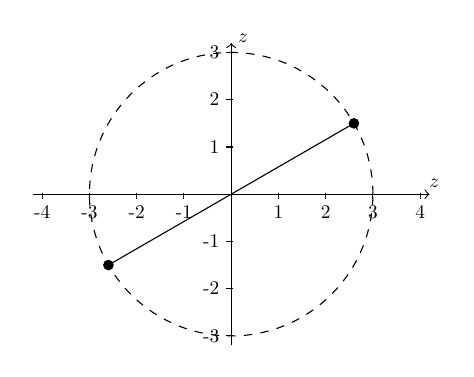
\begin{tikzpicture}[scale=0.6]
	  \draw[->] (-4.2,0) -- (4.2,0) ; \node[above,scale=0.7] at (4.3,0) {$\RE{z}$};
    \draw[->] (0,-3.2) -- (0,3.2) ; \node[right,scale=0.7] at (0,3.3) {$\IM{z}$}; 
		\foreach \x in {-4,-3,-2,-1,1,2,3,4}
     		\draw (\x,1pt) -- (\x,-3pt) node[anchor=north,scale=0.7] {\x};
    \foreach \y in {-3,-2,-1,1,2,3}
     		\draw (1pt,\y) -- (-3pt,\y) node[anchor=east,scale=0.7] {\y};
		\def\r{3}
		\def\theta{pi/3}
		\def\n{2}
		\draw[dashed] (0,0) circle (\r);
		\foreach \ii in {0,1}{
		\draw[\blue] (0,0) -- ({\r*cos(((\theta+2*pi*\ii)/\n) r)},{\r*sin(((\theta+2*pi*\ii)/\n) r)});
		\draw[fill=\blue]  ({\r*cos(((\theta+2*pi*\ii)/\n) r)},{\r*sin(((\theta+2*pi*\ii)/\n) r)}) circle (0.1);
		}
\end{tikzpicture}
\captionof{figure}{Square roots of $z= 9 e^{i\frac{\pi}{3}}$}
\end{center}

\begin{center}
\begin{tikzpicture}[scale=0.6]
	  \draw[->] (-4.2,0) -- (4.2,0) ; \node[above,scale=0.7] at (4.3,0) {$\RE{z}$};
    \draw[->] (0,-3.2) -- (0,3.2) ; \node[right,scale=0.7] at (0,3.3) {$\IM{z}$}; 
		\foreach \x in {-4,-3,-2,-1,1,2,3,4}
     		\draw (\x,1pt) -- (\x,-3pt) node[anchor=north,scale=0.7] {\x};
    \foreach \y in {-3,-2,-1,1,2,3}
     		\draw (1pt,\y) -- (-3pt,\y) node[anchor=east,scale=0.7] {\y};
		\def\r{2}
		\def\theta{3*pi/4}
		\def\n{3}
		\draw[dashed] (0,0) circle (\r);
		\foreach \ii in {0,1,2}{
		\draw[\blue] (0,0) -- ({\r*cos(((\theta+2*pi*\ii)/\n) r)},{\r*sin(((\theta+2*pi*\ii)/\n) r)});
		\draw[fill=\blue]  ({\r*cos(((\theta+2*pi*\ii)/\n) r)},{\r*sin(((\theta+2*pi*\ii)/\n) r)}) circle (0.1);
		}
\end{tikzpicture}
\captionof{figure}{Third roots of $z= \frac{8(-1+i)}{\sqrt{2}}$}
\end{center}

\begin{center}
\begin{tikzpicture}[scale=0.6]
	  \draw[->] (-4.2,0) -- (4.2,0) ; \node[above,scale=0.7] at (4.3,0) {$\RE{z}$};
    \draw[->] (0,-3.2) -- (0,3.2) ; \node[right,scale=0.7] at (0,3.3) {$\IM{z}$}; 
		\foreach \x in {-4,-3,-2,-1,1,2,3,4}
     		\draw (\x,1pt) -- (\x,-3pt) node[anchor=north,scale=0.7] {\x};
    \foreach \y in {-3,-2,-1,1,2,3}
     		\draw (1pt,\y) -- (-3pt,\y) node[anchor=east,scale=0.7] {\y};
		\def\r{1.222844545}
		\def\theta{2.034443936}
		\def\n{4}
		\draw[dashed] (0,0) circle (\r);
		\foreach \ii in {0,1,2,3}{
		\draw[\blue] (0,0) -- ({\r*cos(((\theta+2*pi*\ii)/\n) r)},{\r*sin(((\theta+2*pi*\ii)/\n) r)});
		\draw[fill=\blue]  ({\r*cos(((\theta+2*pi*\ii)/\n) r)},{\r*sin(((\theta+2*pi*\ii)/\n) r)}) circle (0.1);
		}
\end{tikzpicture}
\captionof{figure}{$4$-th roots of $z= -1+2i$}
\end{center}

\begin{center}
\begin{tikzpicture}[scale=0.6]
	  \draw[->] (-4.2,0) -- (4.2,0) ; \node[above,scale=0.7] at (4.3,0) {$\RE{z}$};
    \draw[->] (0,-3.2) -- (0,3.2) ; \node[right,scale=0.7] at (0,3.3) {$\IM{z}$}; 
		\foreach \x in {-4,-3,-2,-1,1,2,3,4}
     		\draw (\x,1pt) -- (\x,-3pt) node[anchor=north,scale=0.7] {\x};
    \foreach \y in {-3,-2,-1,1,2,3}
     		\draw (1pt,\y) -- (-3pt,\y) node[anchor=east,scale=0.7] {\y};
		\def\r{1.174618943}
		\def\theta{2.034443936}
		\def\n{5}
		\draw[dashed] (0,0) circle (\r);
		\foreach \ii in {0,1,2,3,4}{
		\draw[\blue] (0,0) -- ({\r*cos(((\theta+2*pi*\ii)/\n) r)},{\r*sin(((\theta+2*pi*\ii)/\n) r)});
		\draw[fill=\blue]  ({\r*cos(((\theta+2*pi*\ii)/\n) r)},{\r*sin(((\theta+2*pi*\ii)/\n) r)}) circle (0.1);
		}
\end{tikzpicture}
\captionof{figure}{$5$-th roots of $z= -1+2i$}
\end{center}
\end{multicols}
The $n$-th roots of $z = r e^{i\theta}$ are spaced equally in wedges with angle $\frac{2\pi}{n}$ around a circle of radius $r^{\frac{1}{n}}$. 
\end{example}


As a final application of De Moivre's theorem, we can use it to derive some useful trigonometric identities. 


\begin{example}
Consider the case of $n=2$ in De Moivre's Theorem. We get
\begin{align*}
\cos(2\theta)+i\sin(2\theta) &= (\cos(\theta)+i\sin(\theta))^2 \\
&= \cos^2(\theta)-\sin^2(\theta) + i 2\sin(\theta)\cos(\theta) & \text{Expanding}
\end{align*}
In particular, if we equate the real and imaginary parts of the equation, we recover a couple of well-known identities
\begin{align*}
\cos(2\theta) &= \cos^2(\theta)-\sin^2(\theta) \\
\sin(2\theta) &= 2\sin(\theta)\cos(\theta)
\end{align*}
\end{example}

The theorem gives us two trigonometric identities at the same time.

\begin{exercise}{}
\question Prove the identity $\sin(3\theta)=3\cos^2(\theta)\sin(\theta)-\sin^3(\theta)$ using De Moivre's Theorem.
\end{exercise}

\secbreak
\subsection{Complex Arguments in Trigonometric/Hyperbolic Functions}

We have seen that for any real angle $\theta$, {\it Euler's formula} gives 
\begin{equation*}
e^{i\theta} = \cos(\theta) + i \sin(\theta)
\end{equation*}
which can be used to write \( \sin( \theta ), \cos ( \theta) \)
as
\begin{align*}
\cos(\theta) &= \frac{1}{2}\left(e^{i\theta} + e^{-i\theta}\right),\\
\sin(\theta) &= \frac{1}{2i}\left(e^{i\theta} - e^{-i\theta}\right).
\end{align*}
This can, in turn be used to write 
\begin{align*}
\cos(z) &= \frac{1}{2}\left(e^{i z} + e^{-i z}\right),\\
\sin(z) &= \frac{1}{2i}\left(e^{i z} - e^{-iz}\right).
\end{align*}
for {\it complex} arguments $z$.

If we expand the RHS using $z=x+iy$, we find
\[
\cos(z) = \cos(x) \cosh ( y) - i \sin(x) \sinh(y)
\]
and 
\[
\sin(z) = \sin (x) \cosh(y) + i \cos(x) \sinh(y) \, .
\]


This is also true for $\cosh(z), \sinh(z)$ with complex arguments $z$, i.e.
\begin{align*}
\cosh(z) &= \frac{1}{2}\left(e^{z} + e^{- z}\right),\\
\sinh(z) &= \frac{1}{2}\left(e^{ z} - e^{-z}\right).
\end{align*}
with {\it complex} arguments $z=x+iy$.

\begin{example}
Expand \( \cosh (z) \) for \(z=x+iy \).

Since
\begin{align*}
\cosh(z) &= \frac{1}{2}\left(e^{z} + e^{- z}\right) =
 \frac{1}{2}\left(e^{ x+iy} + e^{-x+iy}\right)\\
 &=  \frac{1}{2}\left(e^x (\cos(y) + i \sin(y)) + e^{-x} (\cos(y) - i \sin(y)) \right)\\
 &=  \frac{1}{2}\left((e^x + e^{-x} )\cos(y) + i (e^x - e^{-x} ) \sin(y) \right)\\
 &=   \cosh(x) \cos(y) + i \sinh(x)\sin(y)
\end{align*}

\end{example}


The exponential function can be defined for complex arguments
\[
\exp(z) = \exp(x+iy) = \exp(x)\exp(iy) = \exp(x) \left( \cos(y) + i \sin(y)\right)
\]
which shows that 
\[
\text{Re} \exp(z) = \exp(x) \cos(y), \qquad \text{Im} \exp(z) =  \exp(x) \sin(y) \, .
\]
The Logarithm can also be defined for complex arguments
\[
\Log(z) = \Log\abs{z} + i\Arg{z}
\]
which can be written as
\[
\Log(z) = \frac12\Log(x^2 + y^2) + i \arctan \left( \frac{y}{x} \right) \, .
\]

You might worry that $\Arg{}$, (i.e.  $\arctan$), might lead to complications in the definition of $\Log$ for complex arguments - it does! Disentangling these is for another course.

\secbreak
\subsection{Complex Mappings}

A nice geometrical way to picture complex functions is to think of them as {\it Complex Mappings}. A complex function $w=u+iv = f(z)$ takes the point $z=x+iy$ in the complex plane and {\it maps} it to $u+iv$. 



\begin{example}
Show the effect of considering $w=iz$ as a complex map that acts on the segment
$1\le |z| \le 2$, $35^\circ \le \arg z \le 75^\circ$ in the complex $z$ plane.

If we use polar form, $i = e^{i \frac{\pi}{2}}$, so it represents a (positive, anticlockwise) rotation by $\pi/2$ radians.

I have sneakily used an alternative notation in the figures for Re$(z)$, namely $\Re(z)$, and Im$(z)$, namely $\Im(z)$.


\begin{tikzpicture}[scale=2, >=Latex, line cap=round, line join=round]

% --- annular sector parameters in the z-plane ---
\def\rIn{1}
\def\rOut{2}
\def\aOne{35}   % degrees
\def\aTwo{75}   % degrees

% ------------------ LEFT: z-plane ------------------
\begin{scope}
  % axes
  \draw[->] (-0.2,0) -- (2.35,0) node[below right] {$\Re(z)$};
  \draw[->] (0,-0.2) -- (0,2.35) node[above left] {$\Im(z)$};

  % shaded annular sector:  aOne <= arg z <= aTwo, rIn <= |z| <= rOut
  % Build it as: outer arc from aOne to aTwo, then inner arc back from aTwo to aOne.
  \path[fill=gray!25, draw=none]
    ({\rOut*cos(\aOne)},{\rOut*sin(\aOne)}) arc (\aOne:\aTwo:\rOut)
    -- ({\rIn*cos(\aTwo)},{\rIn*sin(\aTwo)}) arc (\aTwo:\aOne:\rIn)
    -- cycle;

  % boundary curves of the annular sector
  \draw[thick]
    ({\rOut*cos(\aOne)},{\rOut*sin(\aOne)}) arc (\aOne:\aTwo:\rOut);
  \draw[thick]
    ({\rIn*cos(\aOne)},{\rIn*sin(\aOne)}) arc (\aOne:\aTwo:\rIn);

  % radial sides
  \draw[thick]
    ({\rIn*cos(\aOne)},{\rIn*sin(\aOne)}) -- ({\rOut*cos(\aOne)},{\rOut*sin(\aOne)});
  \draw[thick]
    ({\rIn*cos(\aTwo)},{\rIn*sin(\aTwo)}) -- ({\rOut*cos(\aTwo)},{\rOut*sin(\aTwo)});

  % optional dashed quarter arcs for reference
  \draw[dashed] (0,0) ++(0:\rIn) arc (0:90:\rIn);
  \draw[dashed] (0,0) ++(0:\rOut) arc (0:90:\rOut);

  % labels
  \node[above] at (1.1,2.45) {$z$-plane};
  \node[right] at ({\rOut*cos(55)},{\rOut*sin(55)}) {$1<|z|<2$};
  \node at (1.45,0.40) {$35^\circ \le \arg z \le 75^\circ$};
\end{scope}

% mapping arrow between the two diagrams
\draw[->, thick] (2.75,1.15) -- (3.55,1.15) node[midway,above] {$w=iz$};

% ------------------ RIGHT: w-plane ------------------
% Under w = i z, the region is rotated by +90 degrees:
% 35°..75°  --> 125°..165°  (in the second quadrant), radii unchanged.
\begin{scope}[xshift=6.5cm]
  % axes (space into negative real direction)
  \draw[->] (-2.35,0) -- (0.25,0) node[below right] {$\Re(w)$};
  \draw[->] (0,-0.2) -- (0,2.35) node[above left] {$\Im(w)$};

  % mapped angle range
  \pgfmathsetmacro{\bOne}{\aOne+90}
  \pgfmathsetmacro{\bTwo}{\aTwo+90}

  % shaded mapped annular sector
  \path[fill=gray!25, draw=none]
    ({\rOut*cos(\bOne)},{\rOut*sin(\bOne)}) arc (\bOne:\bTwo:\rOut)
    -- ({\rIn*cos(\bTwo)},{\rIn*sin(\bTwo)}) arc (\bTwo:\bOne:\rIn)
    -- cycle;

  % boundary curves
  \draw[thick]
    ({\rOut*cos(\bOne)},{\rOut*sin(\bOne)}) arc (\bOne:\bTwo:\rOut);
  \draw[thick]
    ({\rIn*cos(\bOne)},{\rIn*sin(\bOne)}) arc (\bOne:\bTwo:\rIn);

  % radial sides
  \draw[thick]
    ({\rIn*cos(\bOne)},{\rIn*sin(\bOne)}) -- ({\rOut*cos(\bOne)},{\rOut*sin(\bOne)});
  \draw[thick]
    ({\rIn*cos(\bTwo)},{\rIn*sin(\bTwo)}) -- ({\rOut*cos(\bTwo)},{\rOut*sin(\bTwo)});

  % optional dashed quadrant arcs for reference (now in quadrant II)
  \draw[dashed] (0,0) ++(90:\rIn) arc (90:180:\rIn);
  \draw[dashed] (0,0) ++(90:\rOut) arc (90:180:\rOut);

  % labels
  \node[above] at (-1.1,2.45) {$w$-plane};
  \node[left] at ({\rOut*cos(145)},{\rOut*sin(145)}) {$1<|w|<2$};
  \node at (-1.55,0.75) {$125^\circ \le \arg w \le 165^\circ$};
\end{scope}

\end{tikzpicture}

\end{example}

\newpage

\begin{example}
Show the effect of considering $w=z^2$ as a complex map that acts on the segment
$1\le |z| \le 2$, $35^\circ \le \arg z \le 75^\circ$ in the complex $z$ plane.

Again, polar form is useful. If $z = r e^{i \theta}$, then $w=r^2 e^{2 i \theta}$.

\begin{tikzpicture}[scale=1.2, >=Latex, line cap=round, line join=round]

% --- annular sector parameters in the z-plane ---
\def\rIn{1}
\def\rOut{2}
\def\aOne{35}   % degrees
\def\aTwo{75}   % degrees

% ------------------ LEFT: z-plane ------------------
\begin{scope}
  % axes
  \draw[->] (-0.2,0) -- (2.35,0) node[below right] {$\Re(z)$};
  \draw[->] (0,-0.2) -- (0,2.35) node[above left] {$\Im(z)$};

  % shaded annular sector in z-plane: aOne..aTwo, rIn..rOut
  \path[fill=gray!25, draw=none]
    ({\rOut*cos(\aOne)},{\rOut*sin(\aOne)}) arc (\aOne:\aTwo:\rOut)
    -- ({\rIn*cos(\aTwo)},{\rIn*sin(\aTwo)}) arc (\aTwo:\aOne:\rIn)
    -- cycle;

  % boundary curves
  \draw[thick]
    ({\rOut*cos(\aOne)},{\rOut*sin(\aOne)}) arc (\aOne:\aTwo:\rOut);
  \draw[thick]
    ({\rIn*cos(\aOne)},{\rIn*sin(\aOne)}) arc (\aOne:\aTwo:\rIn);

  % radial sides
  \draw[thick]
    ({\rIn*cos(\aOne)},{\rIn*sin(\aOne)}) -- ({\rOut*cos(\aOne)},{\rOut*sin(\aOne)});
  \draw[thick]
    ({\rIn*cos(\aTwo)},{\rIn*sin(\aTwo)}) -- ({\rOut*cos(\aTwo)},{\rOut*sin(\aTwo)});

  % dashed reference arcs for |z|=1,2 in first quadrant
  \draw[dashed] (0,0) ++(0:\rIn)  arc (0:90:\rIn);
  \draw[dashed] (0,0) ++(0:\rOut) arc (0:90:\rOut);

  % labels
  \node[above] at (1.1,2.45) {$z$-plane};
  \node at (1.45,0.25) {$35^\circ \le \arg z \le 75^\circ$};
  \node[right] at ({\rOut*cos(55)},{\rOut*sin(55)}) {$1<|z|<2$};
\end{scope}

% mapping arrow between the two diagrams
\draw[->, thick] (2.75,2.15) -- (3.55,2.15) node[midway,above] {$w=z^2$};

% ------------------ RIGHT: w-plane ------------------
% Under w = z^2:  |w| = |z|^2 so radii 1..2 map to 1..4,
% and arg(w) = 2 arg(z) so angles 35..75 map to 70..150 degrees.
\begin{scope}[xshift=8cm]
  % axes (need space into negative Re because the image reaches 150 degrees)
  \draw[->] (-4.35,0) -- (4.35,0) node[below left] {$\Re(w)$};
  \draw[->] (0,-0.35) -- (0,4.35) node[above left] {$\Im(w)$};

  \pgfmathsetmacro{\Rin}{\rIn*\rIn}
  \pgfmathsetmacro{\Rout}{\rOut*\rOut}
  \pgfmathsetmacro{\bOne}{2*\aOne}
  \pgfmathsetmacro{\bTwo}{2*\aTwo}

  % shaded image region in w-plane
  \path[fill=gray!25, draw=none]
    ({\Rout*cos(\bOne)},{\Rout*sin(\bOne)}) arc (\bOne:\bTwo:\Rout)
    -- ({\Rin*cos(\bTwo)},{\Rin*sin(\bTwo)}) arc (\bTwo:\bOne:\Rin)
    -- cycle;

  % boundary curves
  \draw[thick]
    ({\Rout*cos(\bOne)},{\Rout*sin(\bOne)}) arc (\bOne:\bTwo:\Rout);
  \draw[thick]
    ({\Rin*cos(\bOne)},{\Rin*sin(\bOne)}) arc (\bOne:\bTwo:\Rin);

  % radial sides
  \draw[thick]
    ({\Rin*cos(\bOne)},{\Rin*sin(\bOne)}) -- ({\Rout*cos(\bOne)},{\Rout*sin(\bOne)});
  \draw[thick]
    ({\Rin*cos(\bTwo)},{\Rin*sin(\bTwo)}) -- ({\Rout*cos(\bTwo)},{\Rout*sin(\bTwo)});

  % dashed reference arcs for |w|=1 and |w|=4 (upper half-plane)
  \draw[dashed] (0,0) ++(0:\Rin)  arc (0:180:\Rin);
  \draw[dashed] (0,0) ++(0:\Rout) arc (0:180:\Rout);

  % labels
  \node[above] at (-2.0,4.55) {$w$-plane};
  \node at (-2.35,0.25) {$70^\circ \le \arg w \le 150^\circ$};
  \node[left] at ({1.05*\Rout*cos(110)},{1.05*\Rout*sin(110)}) {$1<|w|<4$};
\end{scope}

\end{tikzpicture}
\end{example}






\begin{example}
We can use a complex function to convert a circle (with certain properties) to an aerofoil shape. Each dot on the left plot (the $z$ values) is connected to one on the right (the $w$ values) by the formula
\begin{equation*}
\label{eqn:comptrans}
w(z) = \frac{1}{2}\left(z + \frac{1}{z}\right).
\end{equation*}
The highlighted circles and diamonds show where their $z$ values end up on the $w$ value plot.
Note that the circle in the $z$ plane is slightly off-centre.

\begin{minipage}{0.5\textwidth}
\begin{center}
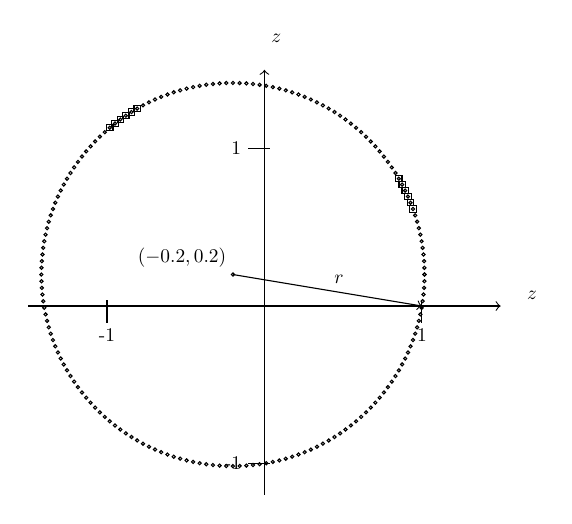
\begin{tikzpicture}[scale=2, declare function={xx(\a,\b) = 1/2*\a*(\a*\a + \b*\b + 1)/(\a*\a + \b*\b); yy(\a,\b) = 1/2*\b*(\a*\a + \b*\b - 1)/(\a*\a + \b*\b);},]
	  \draw[->] (-1.5,0) -- (1.5,0) ; \node[above,scale=0.7] at (1.7,0) {$\RE{z}$};
    \draw[->] (0,-1.2) -- (0,1.5) ; \node[right,scale=0.7] at (0,1.7) {$\IM{z}$}; 
		\foreach \x in {-1,1}
					\draw (\x,1pt) -- (\x,-3pt) node[anchor=north,scale=0.7] {\x};
    \foreach \y in {-1,1}
					\draw (1pt,\y) -- (-3pt,\y) node[anchor=east,scale=0.7] {\y};
	
\def\xshift{0.2} %>0
\def\yshift{0.2} %>0
\def\radius{sqrt((1+\xshift)*(1+\xshift) + (\yshift*\yshift))}
\draw[\blue,->]  (-\xshift,\yshift) -- (1,0) node[midway, above right,scale=0.7] {$r$};
\draw[\blue] (-\xshift,\yshift) circle (0.01); \node[above left,scale=0.7] at  (-\xshift,\yshift) {$(-\xshift, \yshift)$};

\foreach \ii in {0,2,4,...,360} {
\def\real{\radius*cos(\ii)-\xshift}
\def\imag{\radius*sin(\ii)+\yshift}
\draw ({\real},{\imag}) circle (0.01);
}

\foreach \ii in {20,22,...,30} {
\def\real{\radius*cos(\ii)-\xshift}
\def\imag{\radius*sin(\ii)+\yshift}
\draw[\green] ({\real-0.02},{\imag-0.02}) rectangle ++(0.04,0.04);
}

\foreach \ii in {120,122,...,130} {
\def\real{\radius*cos(\ii)-\xshift}
\def\imag{\radius*sin(\ii)+\yshift}
\draw[\red] ({\real-0.02},{\imag-0.02}) rectangle ++(0.04,0.04);
}
\end{tikzpicture}
\end{center}
\end{minipage}%
\begin{minipage}{0.5\textwidth}
\begin{center}
\begin{tikzpicture}[scale=2, declare function={xx(\a,\b) = 1/2*\a*(\a*\a + \b*\b + 1)/(\a*\a + \b*\b); yy(\a,\b) = 1/2*\b*(\a*\a + \b*\b - 1)/(\a*\a + \b*\b);},]
	  \draw[->] (-1.5,0) -- (1.5,0) ; \node[above,scale=0.7] at (1.7,0) {$\RE{w}$};
    \draw[->] (0,-1.2) -- (0,1.5) ; \node[right,scale=0.7] at (0,1.7) {$\IM{w}$}; 
		\foreach \x in {-1,1}
					\draw (\x,1pt) -- (\x,-3pt) node[anchor=north,scale=0.7] {\x};
    \foreach \y in {-1,1}
					\draw (1pt,\y) -- (-3pt,\y) node[anchor=east,scale=0.7] {\y};
	
\def\xshift{0.2} %>0
\def\yshift{0.2} %>0
\def\radius{sqrt((1+\xshift)*(1+\xshift) + (\yshift*\yshift))}
%\draw[\blue,->]  (-\xshift,\yshift) -- (1,0) node[midway, above right,scale=0.7] {$r$};
%\draw[\blue] (-\xshift,\yshift) circle (0.01); \node[above left,scale=0.7] at  (-\xshift,\yshift) {$(-\xshift, \yshift)$};

\foreach \ii in {0,2,4,...,360} {
\def\real{\radius*cos(\ii)-\xshift}
\def\imag{\radius*sin(\ii)+\yshift}
\draw ({xx(\real,\imag)},{yy(\real,\imag)}) circle (0.01);
%\draw ({\real},{\imag}) circle (0.01);
}

\foreach \ii in {20,22,...,30} {
\def\real{\radius*cos(\ii)-\xshift}
\def\imag{\radius*sin(\ii)+\yshift}
\draw[\green] ({xx(\real,\imag)-0.02},{yy(\real,\imag)-0.02}) rectangle ++(0.04,0.04);
%\draw[\green] ({\real-0.02},{\imag-0.02}) rectangle ++(0.04,0.04);
}

\foreach \ii in {120,122,...,130} {
\def\real{\radius*cos(\ii)-\xshift}
\def\imag{\radius*sin(\ii)+\yshift}
\draw[\red] ({xx(\real,\imag)-0.02},{yy(\real,\imag)-0.02}) rectangle ++(0.04,0.04);
%\draw[\red] ({\real-0.02},{\imag-0.02}) rectangle ++(0.04,0.04);
}
\end{tikzpicture}
\end{center}

\end{minipage}%


\(w(z)\) in this example is a {\it complex} function. The argument \(z\) is a complex number and the function returns a complex number \(w(z)\). 




Let us pick apart \( w(z)\) in Cartesian form. 
\begin{align*}
w(z) &= \frac{1}{2}\left(z + \frac{1}{z}\right) = \frac{1}{2}\left(x + i y + \frac{1}{x+iy}\right)\\
     &= \frac{1}{2}\left(x + i y + \frac{x-iy}{x^2+y^2}\right)\\
     &= \frac{1}{2}\left(x + \frac{x}{x^2+y^2} + i \left( y - \frac{y}{x^2+y^2} \right) \right)
\end{align*}

We can see that the {\it complex} function \( w(z)\) may be written using two {\it real}-valued functions of \(x,y\)
\[
w(z) = u(x,y) + i v(x,y)  
\]
where
\[
u(x,y) = x + \frac{x}{x^2+y^2}, \qquad v(x,y) =  y - \frac{y}{x^2+y^2}
\]
This is true in general.
\end{example}

\begin{example}
Let the initial circle now be centred on the origin with radius $R$, i.e. \(|z|=R\) with \(R>0\).  
What is \(w(z)\)?

Parametrize it by
\[
z = R e^{i\theta}, \qquad 0\le \theta < 2\pi .
\]
Then
\begin{align*}
w(z)
&= \frac12\left(z+\frac1z\right)
 = \frac12\left(R e^{i\theta} + \frac{1}{R}e^{-i\theta}\right) \\
&= \frac12\Big((R+\tfrac1R)\cos\theta \;+\; i\,(R-\tfrac1R)\sin\theta\Big).
\end{align*}
Writing \(w=u+iv\), we have
\[
u=\frac{R+\frac1R}{2}\cos\theta,
\qquad
v=\frac{R-\frac1R}{2}\sin\theta.
\]
Eliminating \(\theta\) gives
\[
\frac{u^2}{\left(\frac{R+\frac1R}{2}\right)^2}
+
\frac{v^2}{\left(\frac{|R-\frac1R|}{2}\right)^2}
=1.
\]
Hence the image of the circle \(|z|=R\) under \(w(z)=\tfrac12(z+1/z)\) is an ellipse
centered at the origin, with semiaxes
\[
a=\frac{R+\frac1R}{2} \quad\text{(along the real axis)},\qquad
b=\frac{|R-\frac1R|}{2} \quad\text{(along the imaginary axis)}.
\]
In the special case \(R=1\), the ellipse degenerates to the line segment.
\[
w=\cos\theta\in[-1,1].
\]


% Requires: \usepackage{tikz}
% (and your colour macros \blue,\red,\green or replace them by e.g. blue,red,green)

\begin{minipage}{0.5\textwidth}
\begin{center}
\begin{tikzpicture}[scale=2]
  % axes in the z-plane
  \draw[->] (-1.6,0) -- (1.6,0) ; \node[above,scale=0.7] at (1.8,0) {$\RE{z}$};
  \draw[->] (0,-1.4) -- (0,1.6) ; \node[right,scale=0.7] at (0,1.8) {$\IM{z}$};

  \foreach \x in {-1,1}
    \draw (\x,1pt) -- (\x,-3pt) node[anchor=north,scale=0.7] {\x};
  \foreach \y in {-1,1}
    \draw (1pt,\y) -- (-3pt,\y) node[anchor=east,scale=0.7] {\y};

  % circle |z|=R
  \def\R{1.25}
  \draw[\blue,thick] (0,0) circle (\R);
  \node[above right,scale=0.7] at ({\R/sqrt(2)},{\R/sqrt(2)}) {$|z|=R$};

  % a couple of highlighted arcs on the circle (like your style)
  \foreach \ii in {20,22,...,30} {
    \def\real{\R*cos(\ii)}
    \def\imag{\R*sin(\ii)}
    \draw[\green] ({\real-0.02},{\imag-0.02}) rectangle ++(0.04,0.04);
  }
  \foreach \ii in {120,122,...,130} {
    \def\real{\R*cos(\ii)}
    \def\imag{\R*sin(\ii)}
    \draw[\red] ({\real-0.02},{\imag-0.02}) rectangle ++(0.04,0.04);
  }
\end{tikzpicture}
\end{center}
\end{minipage}%
\begin{minipage}{0.5\textwidth}
\begin{center}
\begin{tikzpicture}[scale=2]
  % axes in the w-plane
  \draw[->] (-1.6,0) -- (1.6,0) ; \node[above,scale=0.7] at (1.8,0) {$\RE{w}$};
  \draw[->] (0,-1.4) -- (0,1.6) ; \node[right,scale=0.7] at (0,1.8) {$\IM{w}$};

  \foreach \x in {-1,1}
    \draw (\x,1pt) -- (\x,-3pt) node[anchor=north,scale=0.7] {\x};
  \foreach \y in {-1,1}
    \draw (1pt,\y) -- (-3pt,\y) node[anchor=east,scale=0.7] {\y};

  % parameters: image ellipse semi-axes
  \def\R{1.25}
  \pgfmathsetmacro{\a}{0.5*(\R + 1/\R)}   % semi-axis on Re(w)
  \pgfmathsetmacro{\b}{0.5*abs(\R - 1/\R)}% semi-axis on Im(w)

  % draw the image ellipse
  \draw[\blue,thick] (0,0) ellipse ({\a} and {\b});
  \node[above right,scale=0.7] at ({\a/sqrt(2)},{\b/sqrt(2)}) {$w=\tfrac12(z+1/z)$};

  % optional: show the focal points (always at \pm 1)
  %\draw (1,0) circle (0.01); \draw (-1,0) circle (0.01);
  %\node[below,scale=0.7] at (1,0) {$1$};
  %\node[below,scale=0.7] at (-1,0) {$-1$};

  % matching highlighted arcs on the ellipse (same theta ranges)
  \foreach \ii in {20,22,...,30} {
    \def\real{\a*cos(\ii)}
    \def\imag{\b*sin(\ii)}
    \draw[\green] ({\real-0.02},{\imag-0.02}) rectangle ++(0.04,0.04);
  }
  \foreach \ii in {120,122,...,130} {
    \def\real{\a*cos(\ii)}
    \def\imag{\b*sin(\ii)}
    \draw[\red] ({\real-0.02},{\imag-0.02}) rectangle ++(0.04,0.04);
  }
\end{tikzpicture}
\end{center}
\end{minipage}%
    
\end{example}

\begin{exercise}{}
    Consider the {\it quadratic map}, $f(z) = z^2 +c$ where $c=a+ib$ (with $a,b$ real) is a complex constant. 
    
    What is $f(z)$ when written in terms of real functions $g,h$. i.e. $f(z)= f(x+iy) = g(x,y) + i h(x,y)$? 
\end{exercise}

\begin{solution}
    Substitute $z=x+iy$ into $f(z)=z^2 + c$ and gather the real and imaginary parts:
    \begin{eqnarray*}
        f(z) &= f(z+iy) = (x+iy)^2 + a + ib \\
        &= (x^2 - y^2 + a) + i (2  xy +b) 
    \end{eqnarray*}
   hence $g(x,y) = x^2 - y^2 + a$ and $h(x,y) = 2  xy +b $
\end{solution}

%------------------------------------------------------------
\subsection{Iterating complex maps}

One of the most striking uses of complex numbers is in \emph{complex dynamics}, where we repeatedly apply a map
\[
z_{n+1}=f(z_n),\qquad n=0,1,2,\dots
\]
starting from some initial value \(z_0\in\mathbf{C}\).  The resulting sequence \(\{z_n\}\) is called the \emph{orbit} of \(z_0\).
Even very simple choices of \(f\) can produce complicated behaviour: orbits may converge to a fixed point, fall into a
periodic cycle, or escape to infinity.

\medskip
We have just encountered the \emph{quadratic map}
\[
f_c(z)=z^2+c,
\]
where \(c\in\mathbf{C}\) is a complex parameter.  A useful practical fact is the \emph{escape radius}:
if at some step \(|z_n|>2\) (when \( | c | < 2 \)), then the orbit will diverge to infinity (so we do not need to keep iterating).

\begin{example}
If we consider a few iterates in the complex plane: Take \(c=-0.123+0.745\,i\) and start at \(z_0=0\). The first few iterates are
\[
z_1=c,\qquad
z_2\approx -0.6629+0.5617\,i,\qquad
z_3\approx 8.9\times10^{-4}+2.6\times10^{-4}\,i,
\]
and then the orbit returns close to \(z_1\) and \(z_2\) again.
\end{example}


\begin{example}
Julia sets (bounded starting points):
Fix \(c\in\mathbf{C}\).  The \emph{filled Julia set} \(K_c\) is the set of starting values 
\(z_0\) whose orbits under
\(z_{n+1}=z_n^2+c\) stay bounded.  (The \emph{Julia set} \(J_c\) is the boundary of \(K_c\).)
The picture below is a coarse ``escape-time'' plot for \(c=-1\): points \(z_0\) that do \emph{not} escape after a fixed
number of iterations (200) are drawn as yellow dots.

\begin{center}
\includegraphics[width=0.5\textwidth]{julia_c_minus1.png}
\end{center}
\end{example}

\begin{example}

The Mandelbrot set (bounded parameters):

Instead of fixing \(c\) and varying \(z_0\), we can fix the starting point \(z_0=0\) and vary the parameter \(c\).
The \emph{Mandelbrot set} \(M\) is the set of parameters \(c\) for which the orbit of \(0\) under \(z_{n+1}=z_n^2+c\)
remains bounded.  The plot below is again an escape-time picture (very low resolution), now in the \(c\)-plane.

\begin{center}
\includegraphics[width=0.5\textwidth]{mandelbrot.png}
\end{center}
\end{example}